\chapter{Setup}
\label{chap:setup}

This chapter is about the first task at hand.
We want to find an archetypal model for the peculiar behavior of the original model.
For this, we first analyze the original model function and note the characteristics.
After that, we construct different models with different characteristics and analyze their behavior as outlined in \Cref{chap:approach}.

\section{Characteristics}
\label{sec:setup.char}

In this section, we will analyze the original model function and note the characteristics.
The first kind of characteristics is the shape of the function.
After that, we will examine the effects that the parameters have on the shape of the function.

\subsection{Function Shape}

\begin{figure}
	\centering
	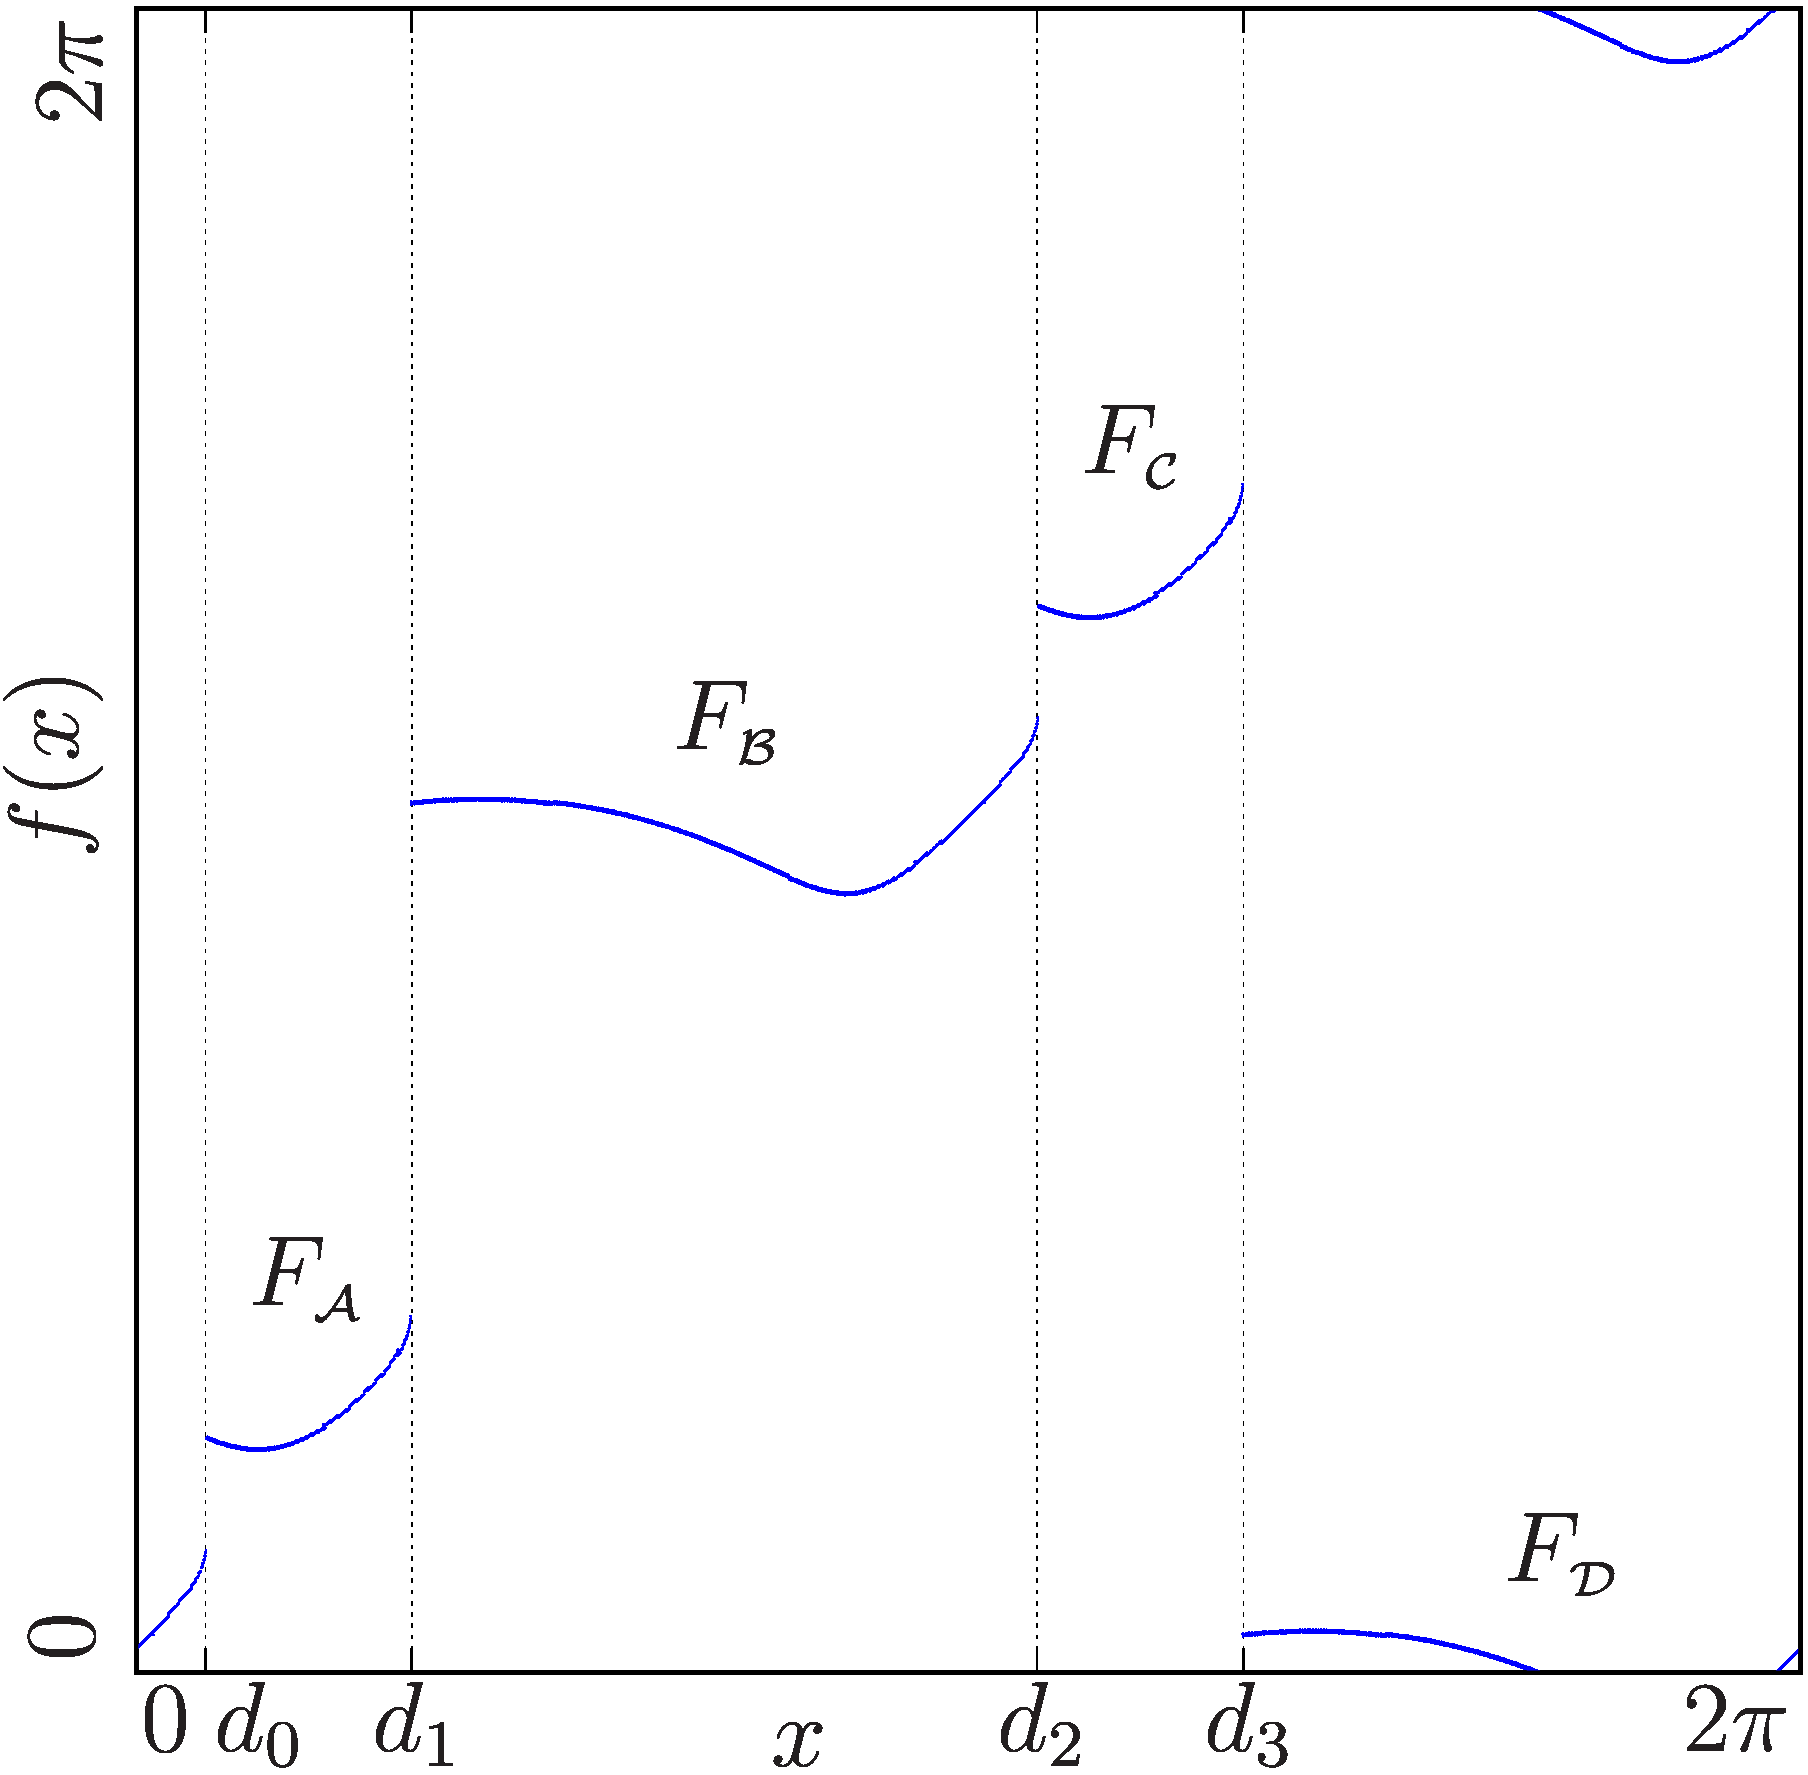
\includegraphics[width=.5 \textwidth]{../Figures/5/5.1/illustration.png}
	\caption[Shape of the original model function]{
		The shape of the original model function at the parameter values $E_0 = 15$ and $\chi_0 = 0.2$.
	}
	\label{fig:setup.char.shape}
\end{figure}

This section is concerned with the overall shape and number of branches of the original model function.

\Cref{fig:setup.char.shape} shows the shape of the original model function.
One can immediately see that the model function has 4 branches.
This is also evident from the model definition given in \Cref{sec:state.og.def}.
Also, we know from \Cref{sec:state.og.dynamics} that the model has the symmetry described by \Cref{equ:state.og.sym}.
So the branches $F_\A$ and $F_\C$ are identical.
The same is true for the branches $F_\B$ and $F_\D$.

There are no fixed points in the parameter regions that this thesis is concerned with.
That means, the function is always larger than the bisector $y=x$.
Also, for the most part the slope of the function is not steep.
Meaning that the absolute value of the model functions derivative is below $1$ for a majority of the state space.
A model where the absolute value of the derivative of its model function is below $1$ for the whole state space is called contractive.
In such a model, every fixed point and cycle is stable.

\subsection{Parameter Effects}
\label{sec:setup.char.paramfx}

This section is concerned with the other types of characteristics, the effects of the parameters of the model on the shape of the model function.
First, it analyzes the combined parameter effects along a chain of parameter regions assocoated with cycles the same period.
After that, it analyzes the isolated effects of the single parameters and decomposes the combined effects into the isolated effects.

\subsection{Combined Effects of Parameters}
\label{sec:setup.char.paramfx.combined}

To replicate the dynamics seen in the model, it is helpful to know, how the model changes along the chains of parameter regions that are associated with cycles of the same period.
This section therefore analyzes the model function at different points in different chains.
\Cref{fig:setup.char.evolution.map} indicates the points used for this analysis.
\Cref{fig:setup.char.evolution.12} shows, how the model function changes along the chain of parameter regions associated with cycles of period 12.
In the figure, there are three functions $F^{A_12}, F^{B_12},$ and $F^{C_12}$.
The function $F^{A_{12}}$ is the model function with the parameters $E_0 = 15.9, \chi_0 = 0.11$.
These parameter values are marked with the point $A_{12}$ in \Cref{fig:setup.char.evolution.map}.
The function $F^{B_{12}}$ is the model function with the parameters $E_0 = 17.07, \chi_0 = 0.182$.
And the function $F^{C_{12}}$ is the model function with the parameters $E_0 = 18.5, \chi_0 = 0.27$.
The parameter values are marked accordingly in \Cref{fig:setup.char.evolution.map}.

\begin{figure}
	\centering
	\subfloat[Points]{
		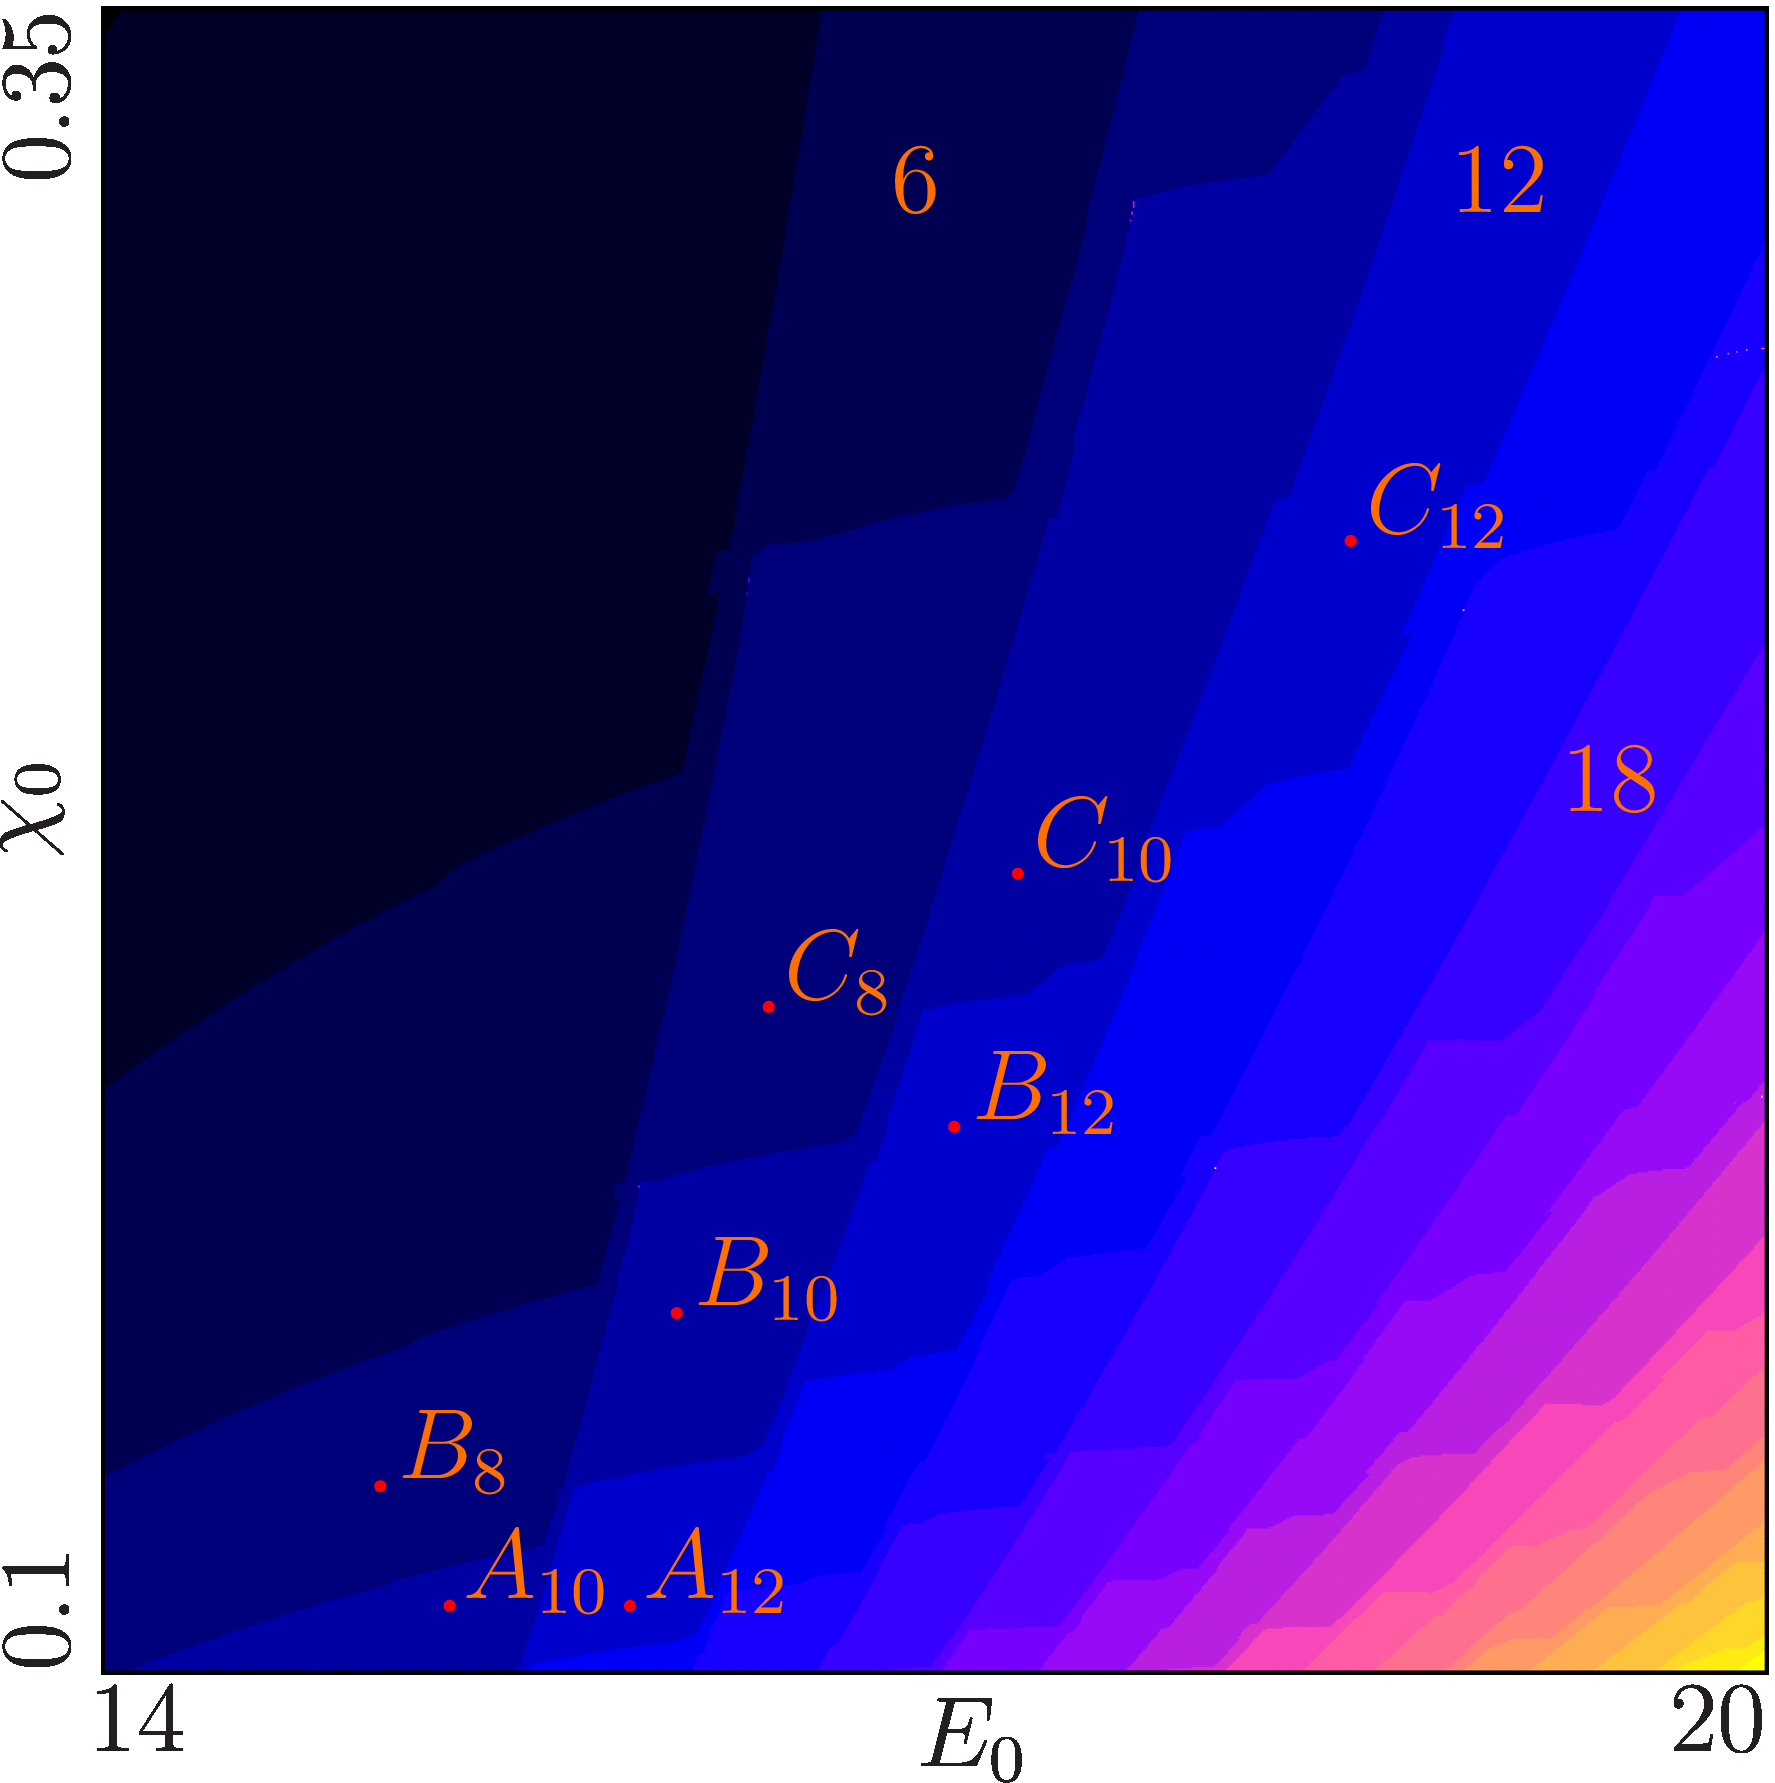
\includegraphics[width=.4 \textwidth]{../Figures/5/5.2a/result.png}
		\label{fig:setup.char.evolution.map}
	}
	\subfloat[Period $12$]{
		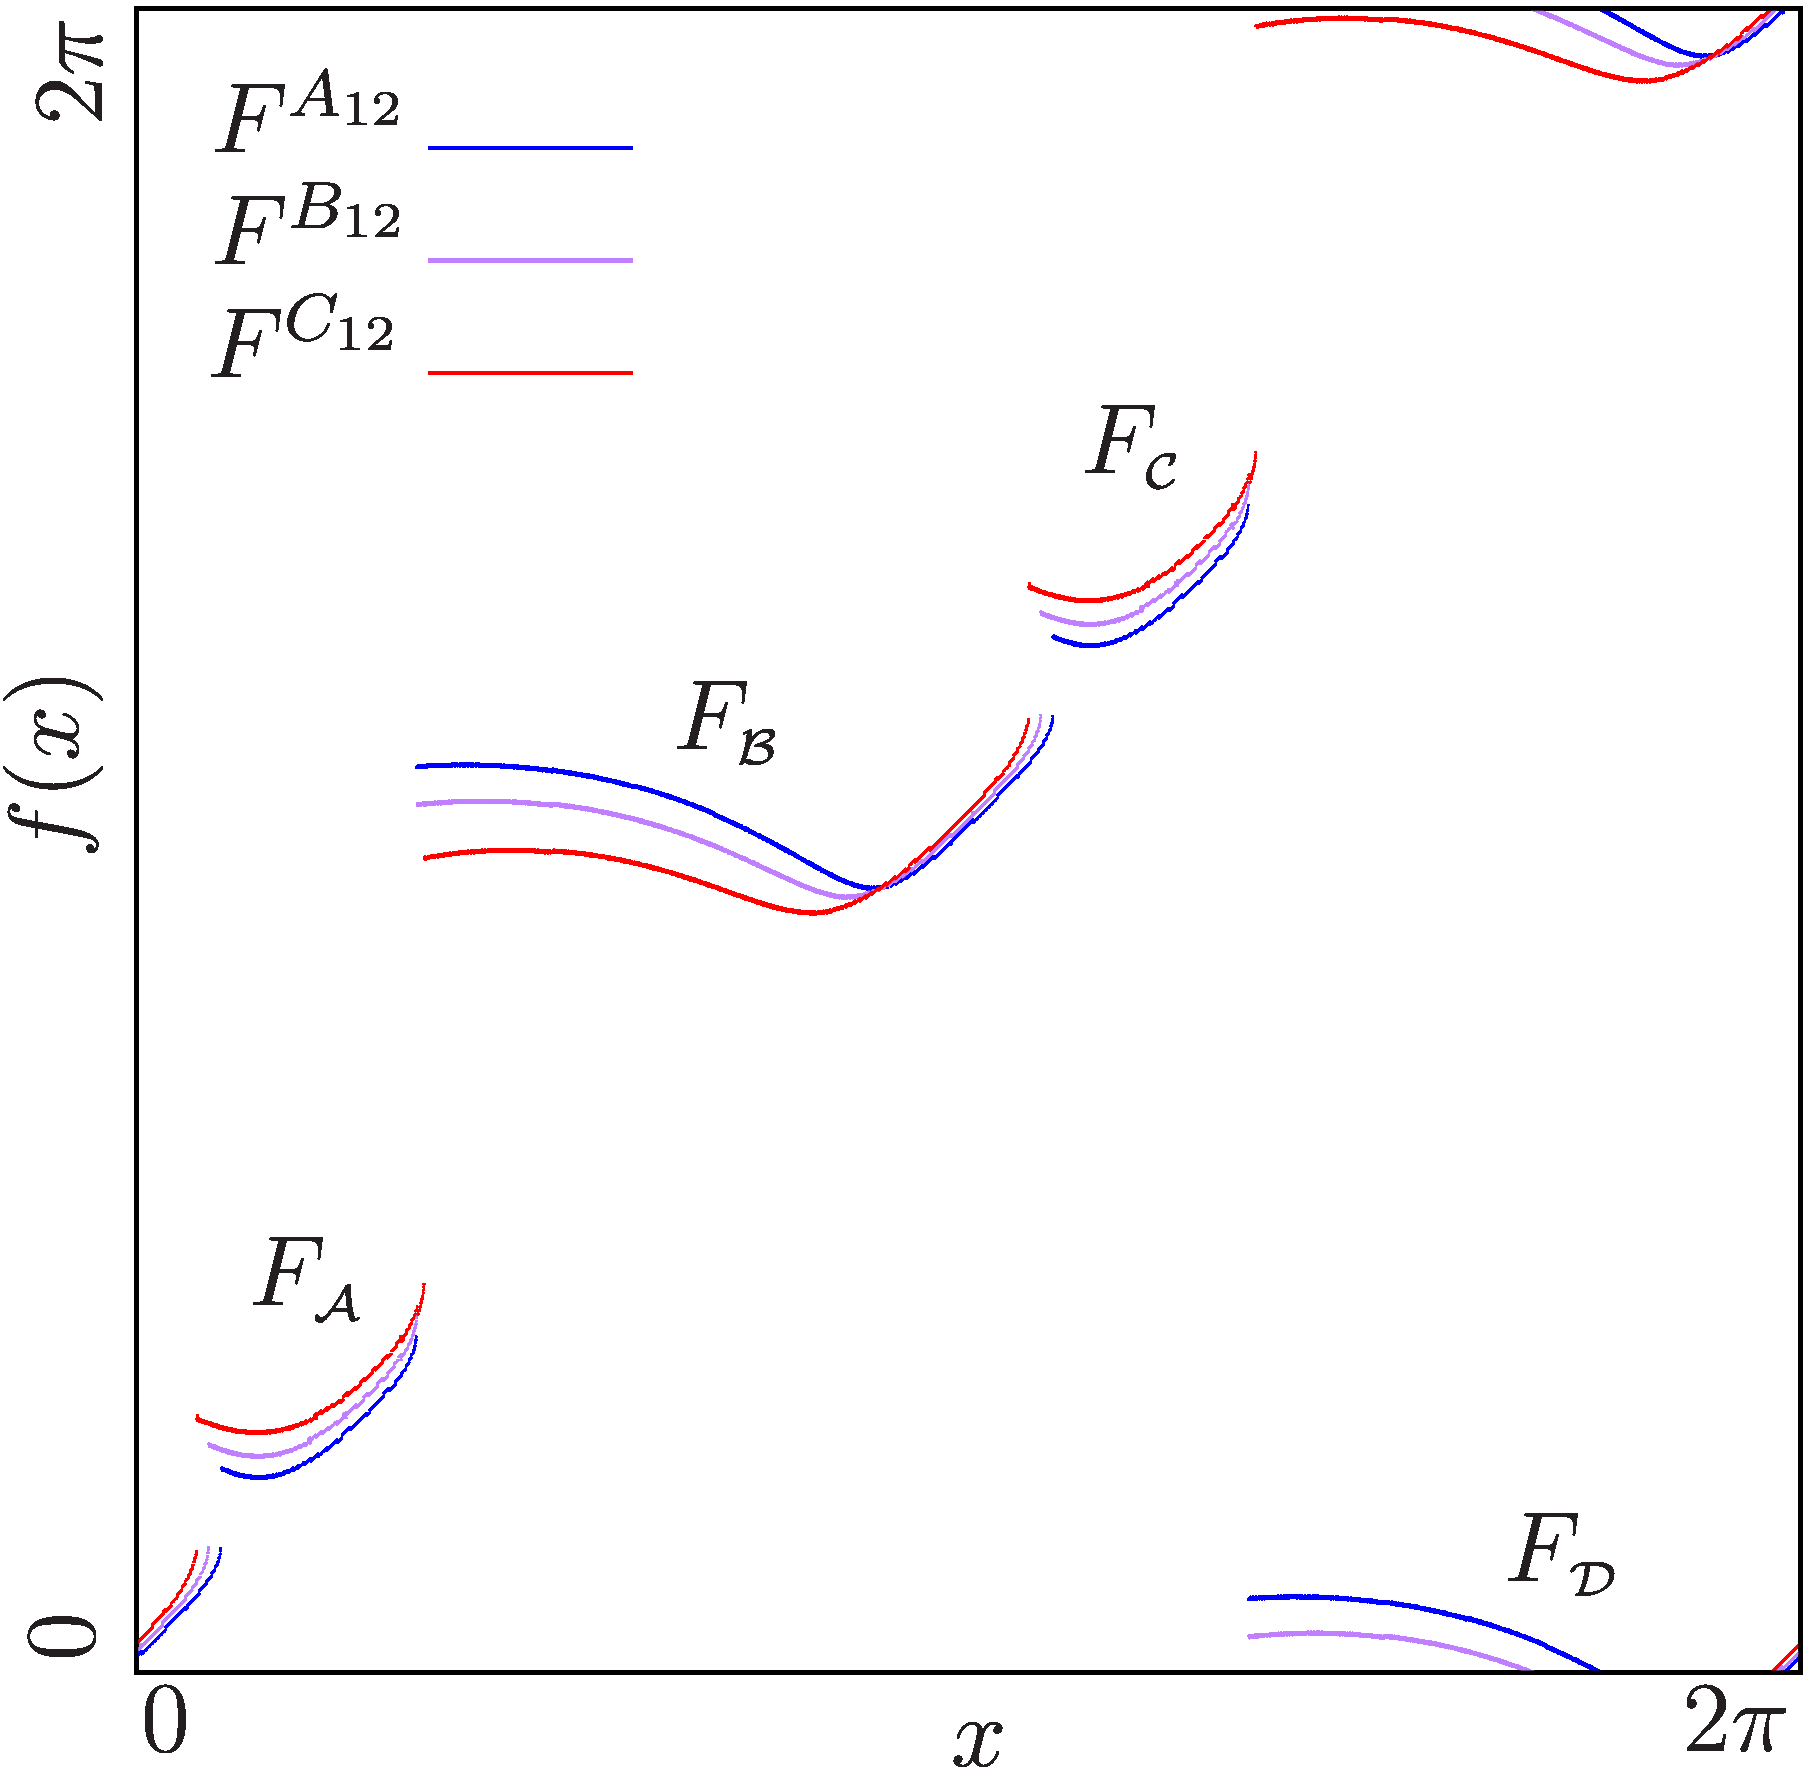
\includegraphics[width=.4 \textwidth]{../Figures/5/5.2b/illustration.png}
		\label{fig:setup.char.evolution.12}
	} \\
	\subfloat[Period $10$]{
		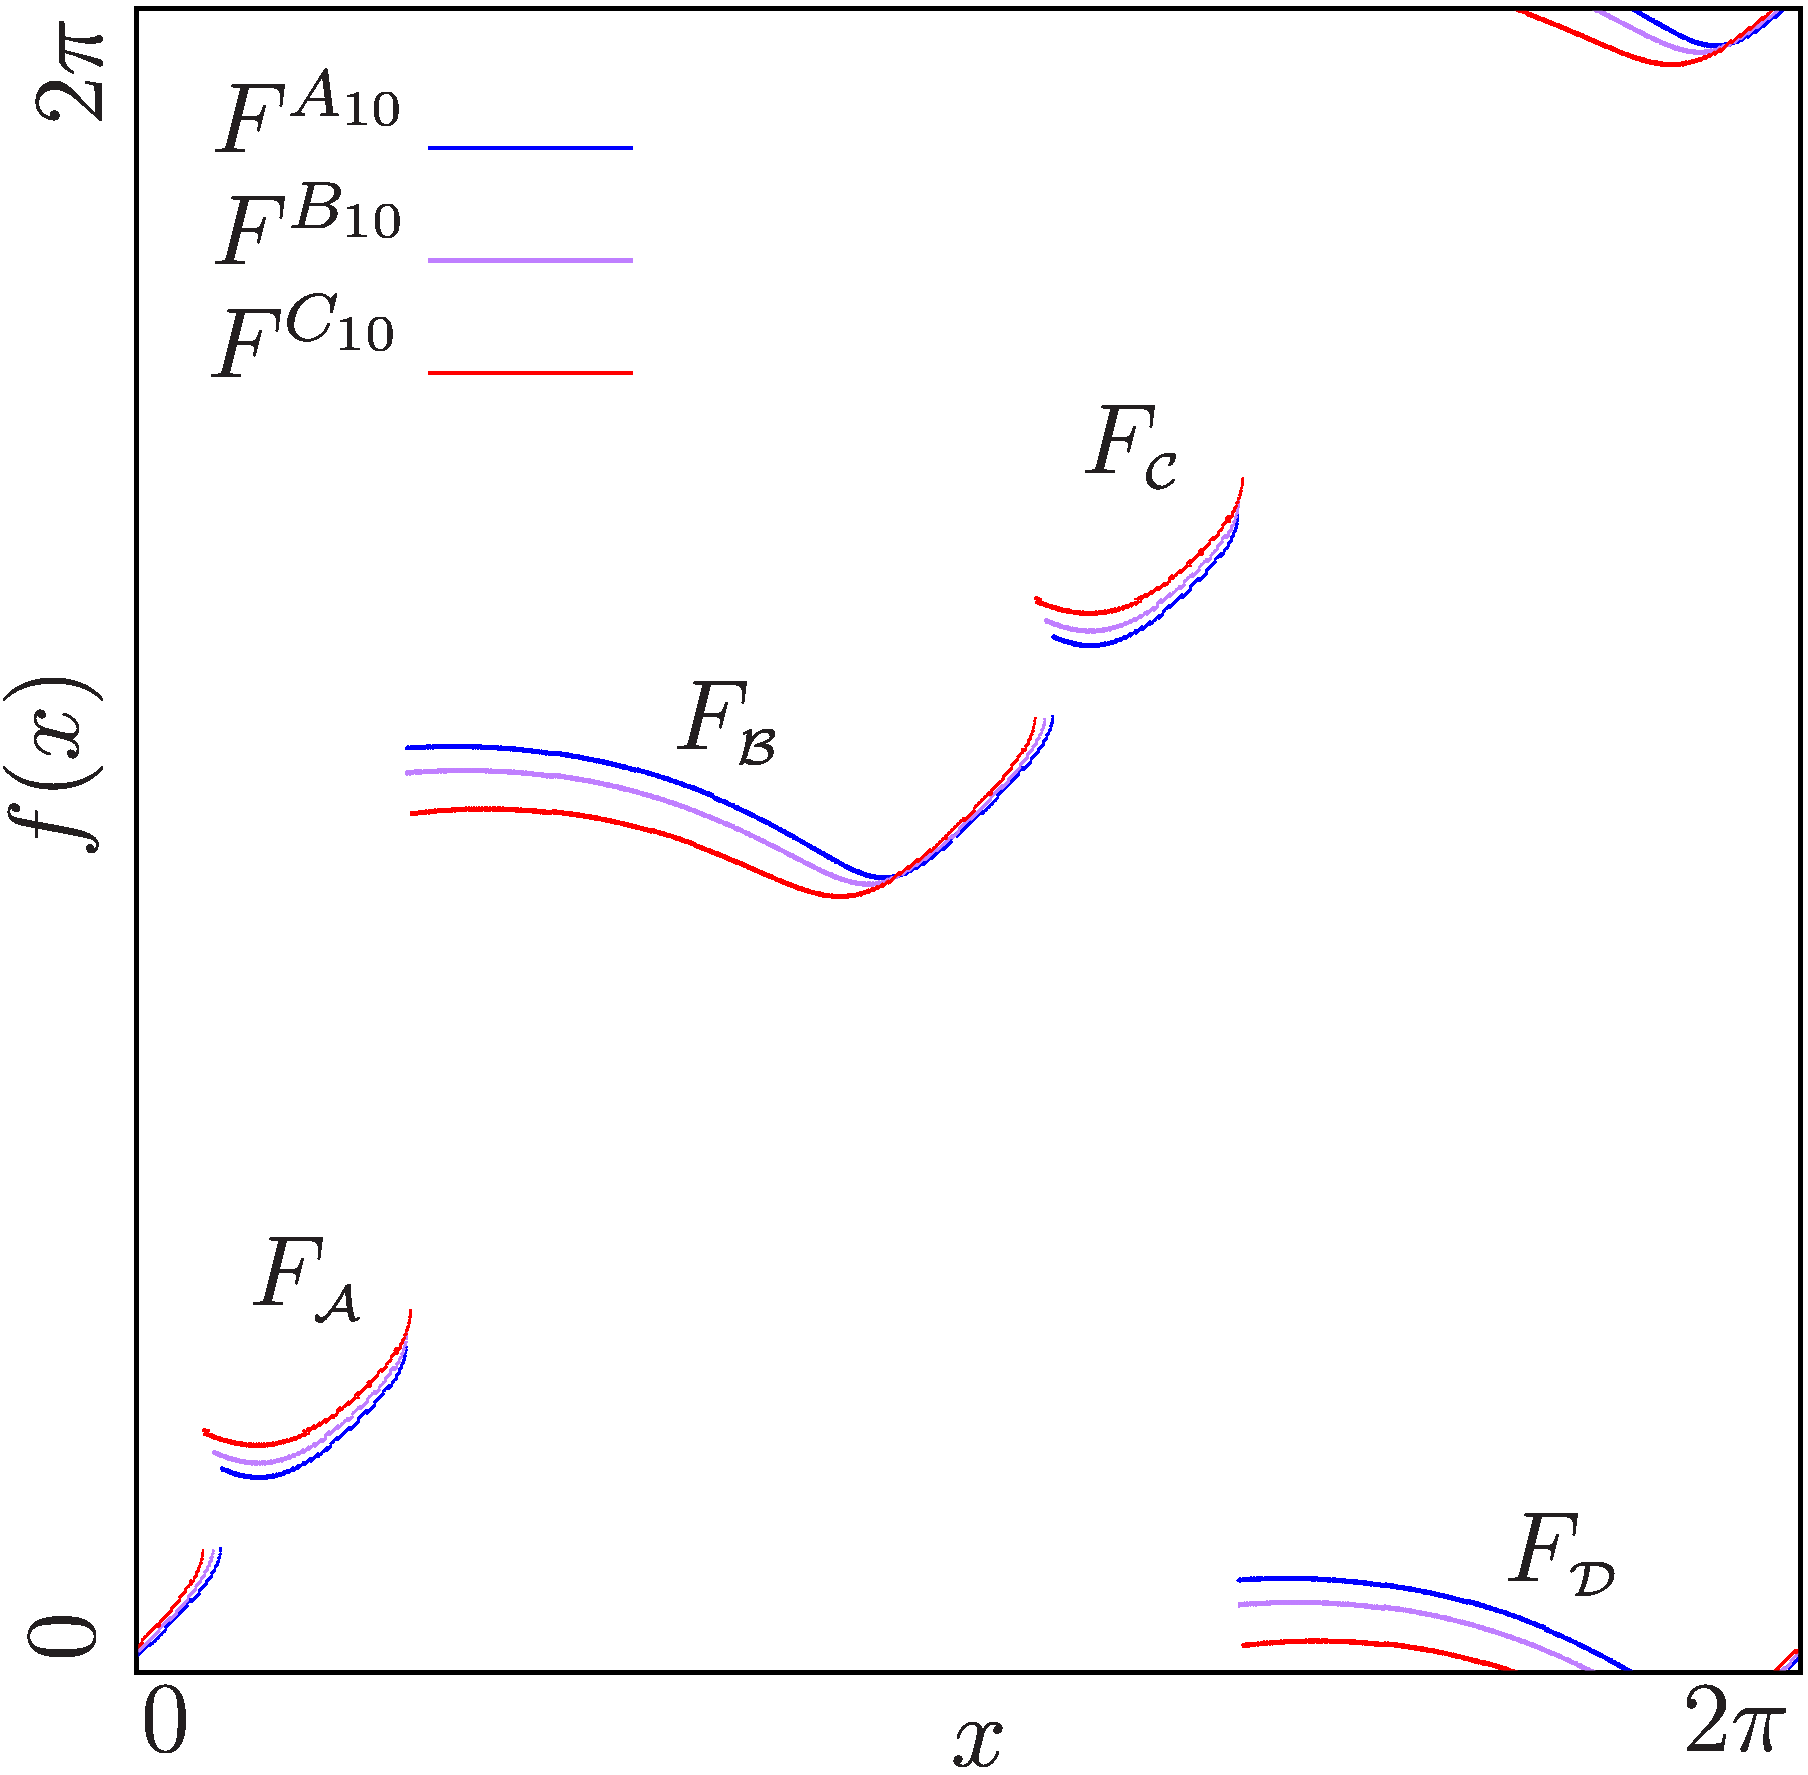
\includegraphics[width=.4 \textwidth]{../Figures/5/5.2c/illustration.png}
		\label{fig:setup.char.evolution.10}
	}
	\subfloat[Period $8$]{
		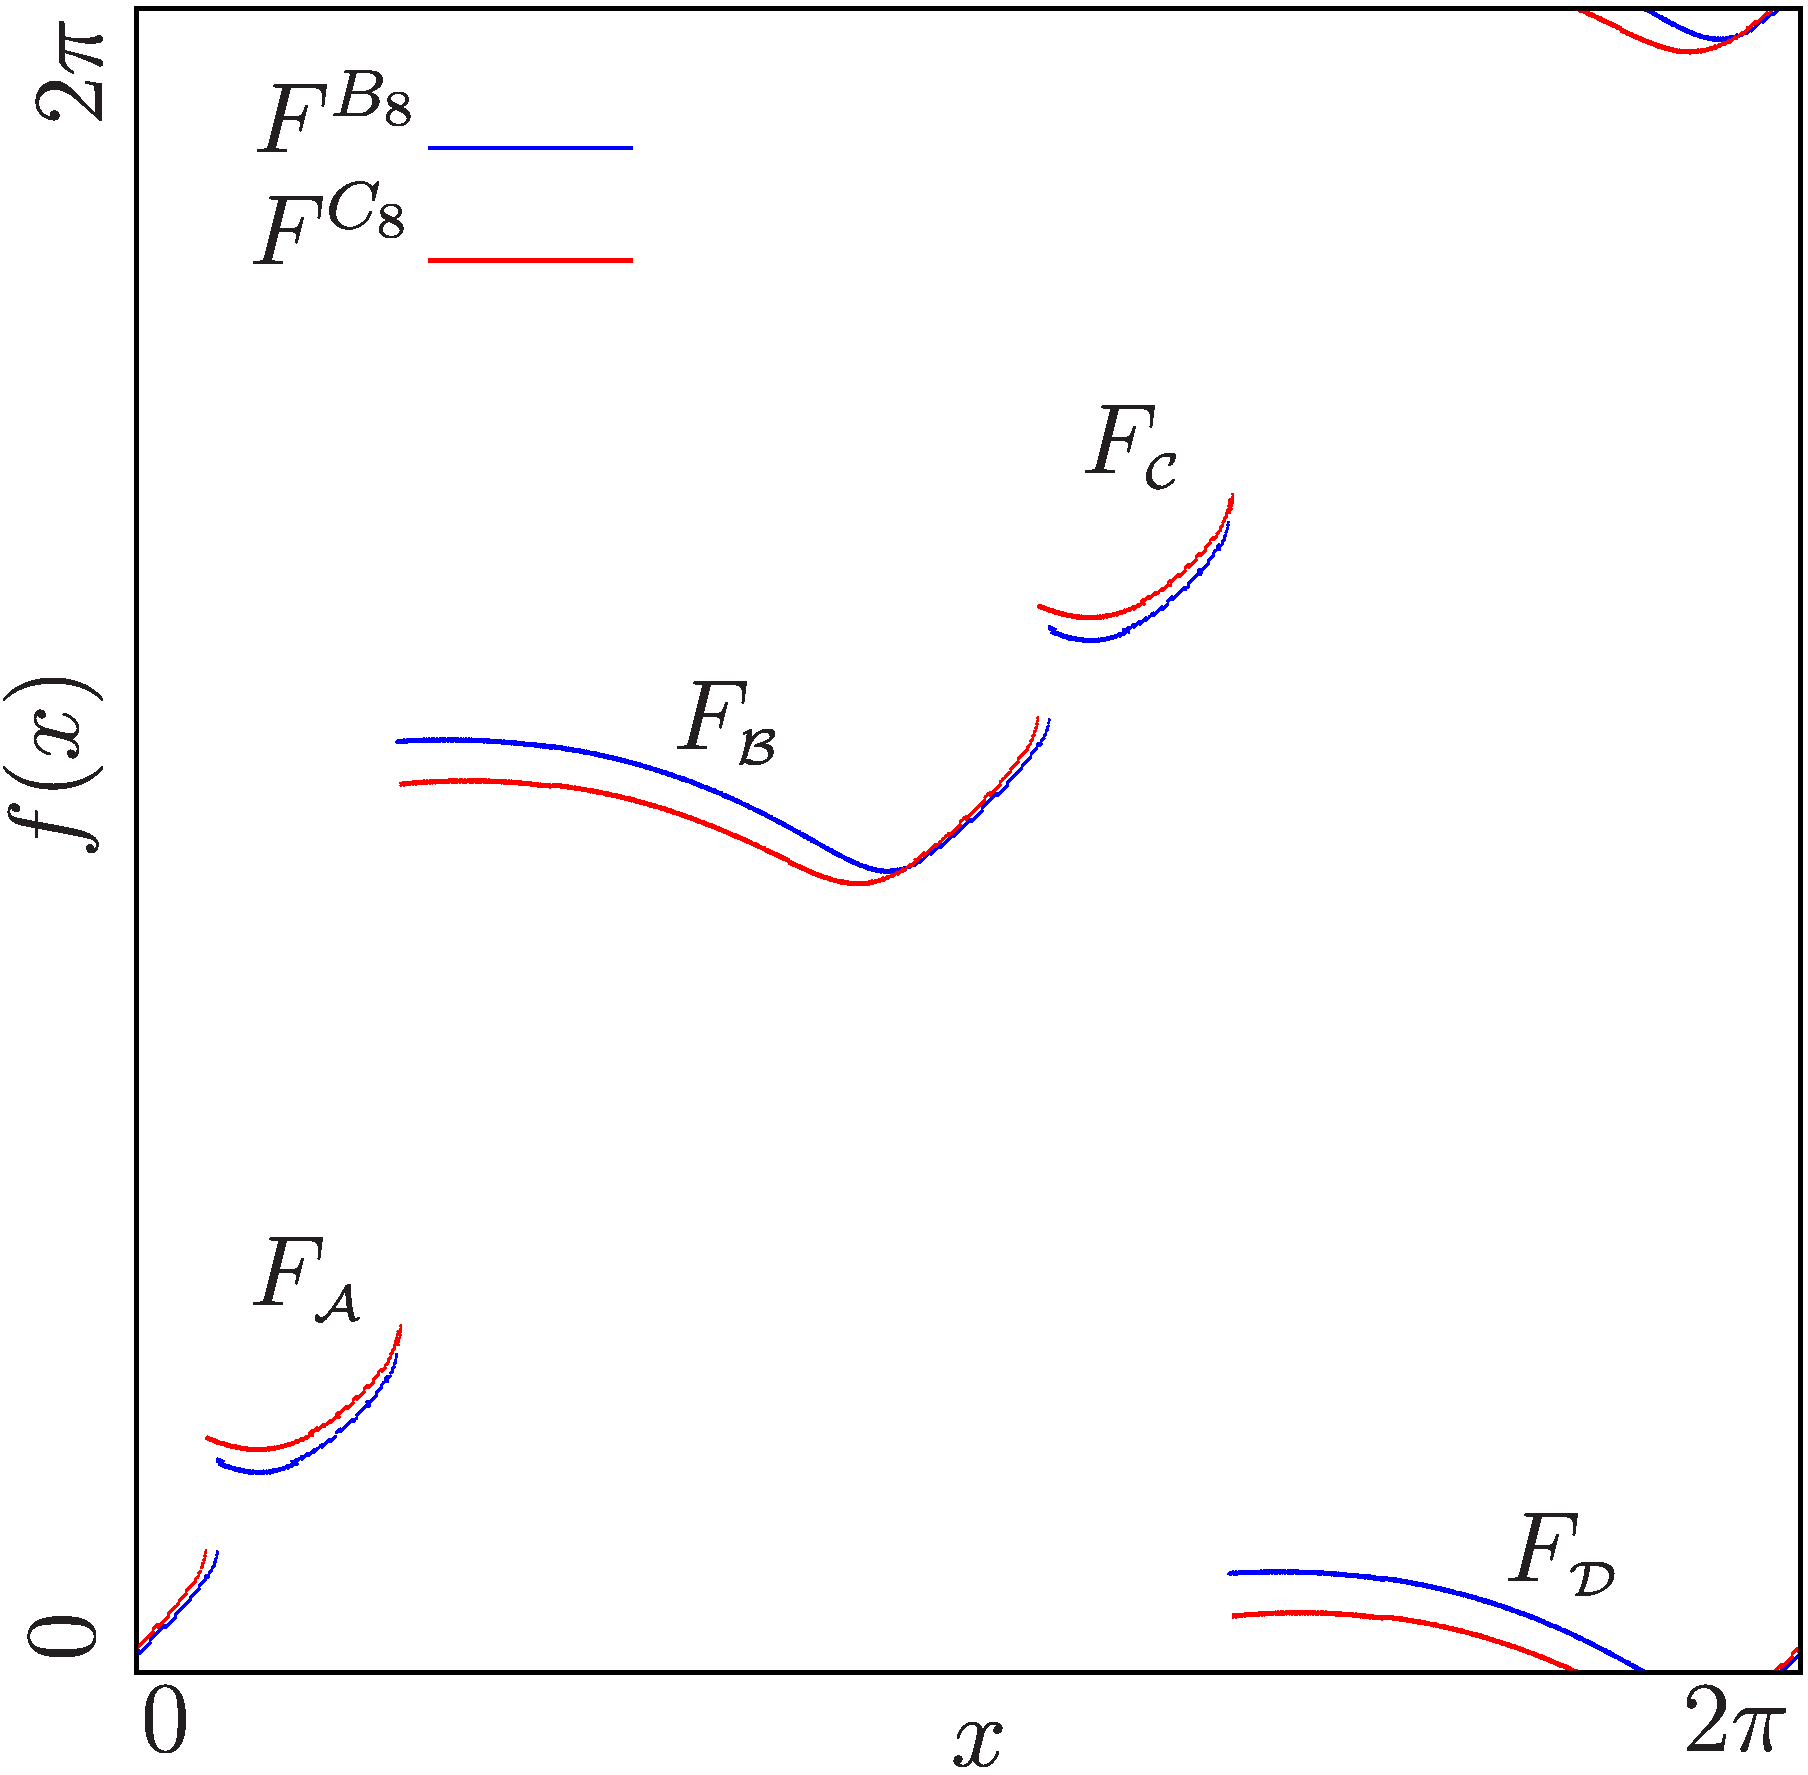
\includegraphics[width=.4 \textwidth]{../Figures/5/5.2d/illustration.png}
		\label{fig:setup.char.evolution.08}
	}
	\caption[The effects of the parameters on the original model function]{
		The effects of the parameters on the original model function illustrated by plotting the model function at different parameter values.
		The parameters $\beta = 1, f = 150, L = 4.2 \cdot 10^{-3}, R = 2, V_m = 5,$ and $\mu = 0.5$ are fixed.
		(a) shows a 2D scan of the periods associated with parameter regions in the original model.
		The parameters $E_0$ and $\chi_0$ are varied in the ranges $[14, 20]$ and $[0.1, 0.35]$.
		The points in this scan mark the parameter values used for plotting the model function in (b), (c), and (d).
		(b) shows the evolution of the shape of the model function along the chain of parameter regions associated with the period 12.
		The function $F^{A_{12}}$ is the model function with the parameter values at the point $A_{12}$ where $E_0 = 15.9$ and $\chi_0 = 0.11$,
		$F^{B_{12}}$ at the point $B_{12}$ where $E_0 = 17.07$ and $\chi_0 = 0.182$,
		and $F^{C_{12}}$ at the point $C_{12}$ where $E_0 = 18.5$ and $\chi_0 = 0.27$.
		(c) shows the evolution of the shape of the model function along the chain of parameter regions associated with the period 10.
		Here, $F^{A_{10}}$ is the model function with the parameters at the point $A_{10}$ where $E_0 = 15.25$ and $\chi_0 = 0.11$,
		$F^{B_{10}}$ at the point $B_{10}$ where $E_0 = 16.07$ and $\chi_0 = 0.154$,
		and $F^{C_{10}}$ at the point $C_{10}$ where $E_0 = 17.3$ and $\chi_0 = 0.22$.
		And (d) shows the evolution of the shape of the model function along the chain of parameter regions associated with the period 8.
		Here, $F^{B_8}$ is the model function with the parameter values at the point $B_8$ where $E_0 = 15$ and $\chi_0 = 0.128$,
		and $F^{C_8}$ at the point $C_8$ where $E_0 = 16.4$ and $\chi_0 = 0.2$.
	}
	\label{fig:setup.char.evolution.combined}
\end{figure}

The most notable changes are the following.
\begin{enumerate}
	\item The values of the whole branches $F_\A$ and $F_\C$ get larger.
	      This change is most notable at the left borders of the branches.
	      The values on the left sides of the branches are affected more by this change than the values on the right sides.
	\item The values on the left sides of the branches $F_\B$ and $F_\D$ get smaller while the values on the right sides are not affected much.
	\item The local minima of the branches $F_\B$ and $F_\D$ move to the left, and their values get smaller.
\end{enumerate}
One smaller change is that the border between branches $F_\B$ and $F_\C$ moves left.
Note that the same change happens to the border between the branches $F_\D$ and $F_\A$ due to the symmetry of the function.

The same effects can be observed in the chains of parameter regions associated with cycles of periods $10$ and $8$, respectively.
For the chain of parameter regions associated with cycles of period $10$, the model function is plotted in \Cref{fig:setup.char.evolution.10} at the three points $A_{10}, B_{10},$ and $C_{10}$ marked in \Cref{fig:setup.char.evolution.map}.
Again, the values of the whole branches $F_\A$ and $F_\C$ are larger in $F^{C_{10}}$ than they are in $F^{A_{10}}$.
And the values on the left sides of the branches $F_\B$ and $F_\D$ are smaller in $F^{C_{10}}$ than they are in $F^{A_{10}}$.
Also, the local minima on those branches move left and down.
For the chain of parameter regions associated with cycles of period $8$, the model function is plotted in \Cref{fig:setup.char.evolution.08} at the two points $B_8$ and $C_8$ marked in \Cref{fig:setup.char.evolution.map}.
And the values of the branches undergo the same changes again from the model function $F^{B_8}$ to $F^{C_8}$.

\subsection{Individual Effects of Parameters}
\label{sec:setup.char.paramfx.individual}

The effects of the parameters described above, always include a change in both parameters $E_0$ and $\chi_0$.
To reproduce the bifurcation structures, it is important to know which effects on the function each parameter has individually.
This section focuses on the isolated effects of each parameter by fixing one of the parameters and only varying the other one and observing the effects of this parameter on the shape of the model function.

\begin{figure}
	\centering
	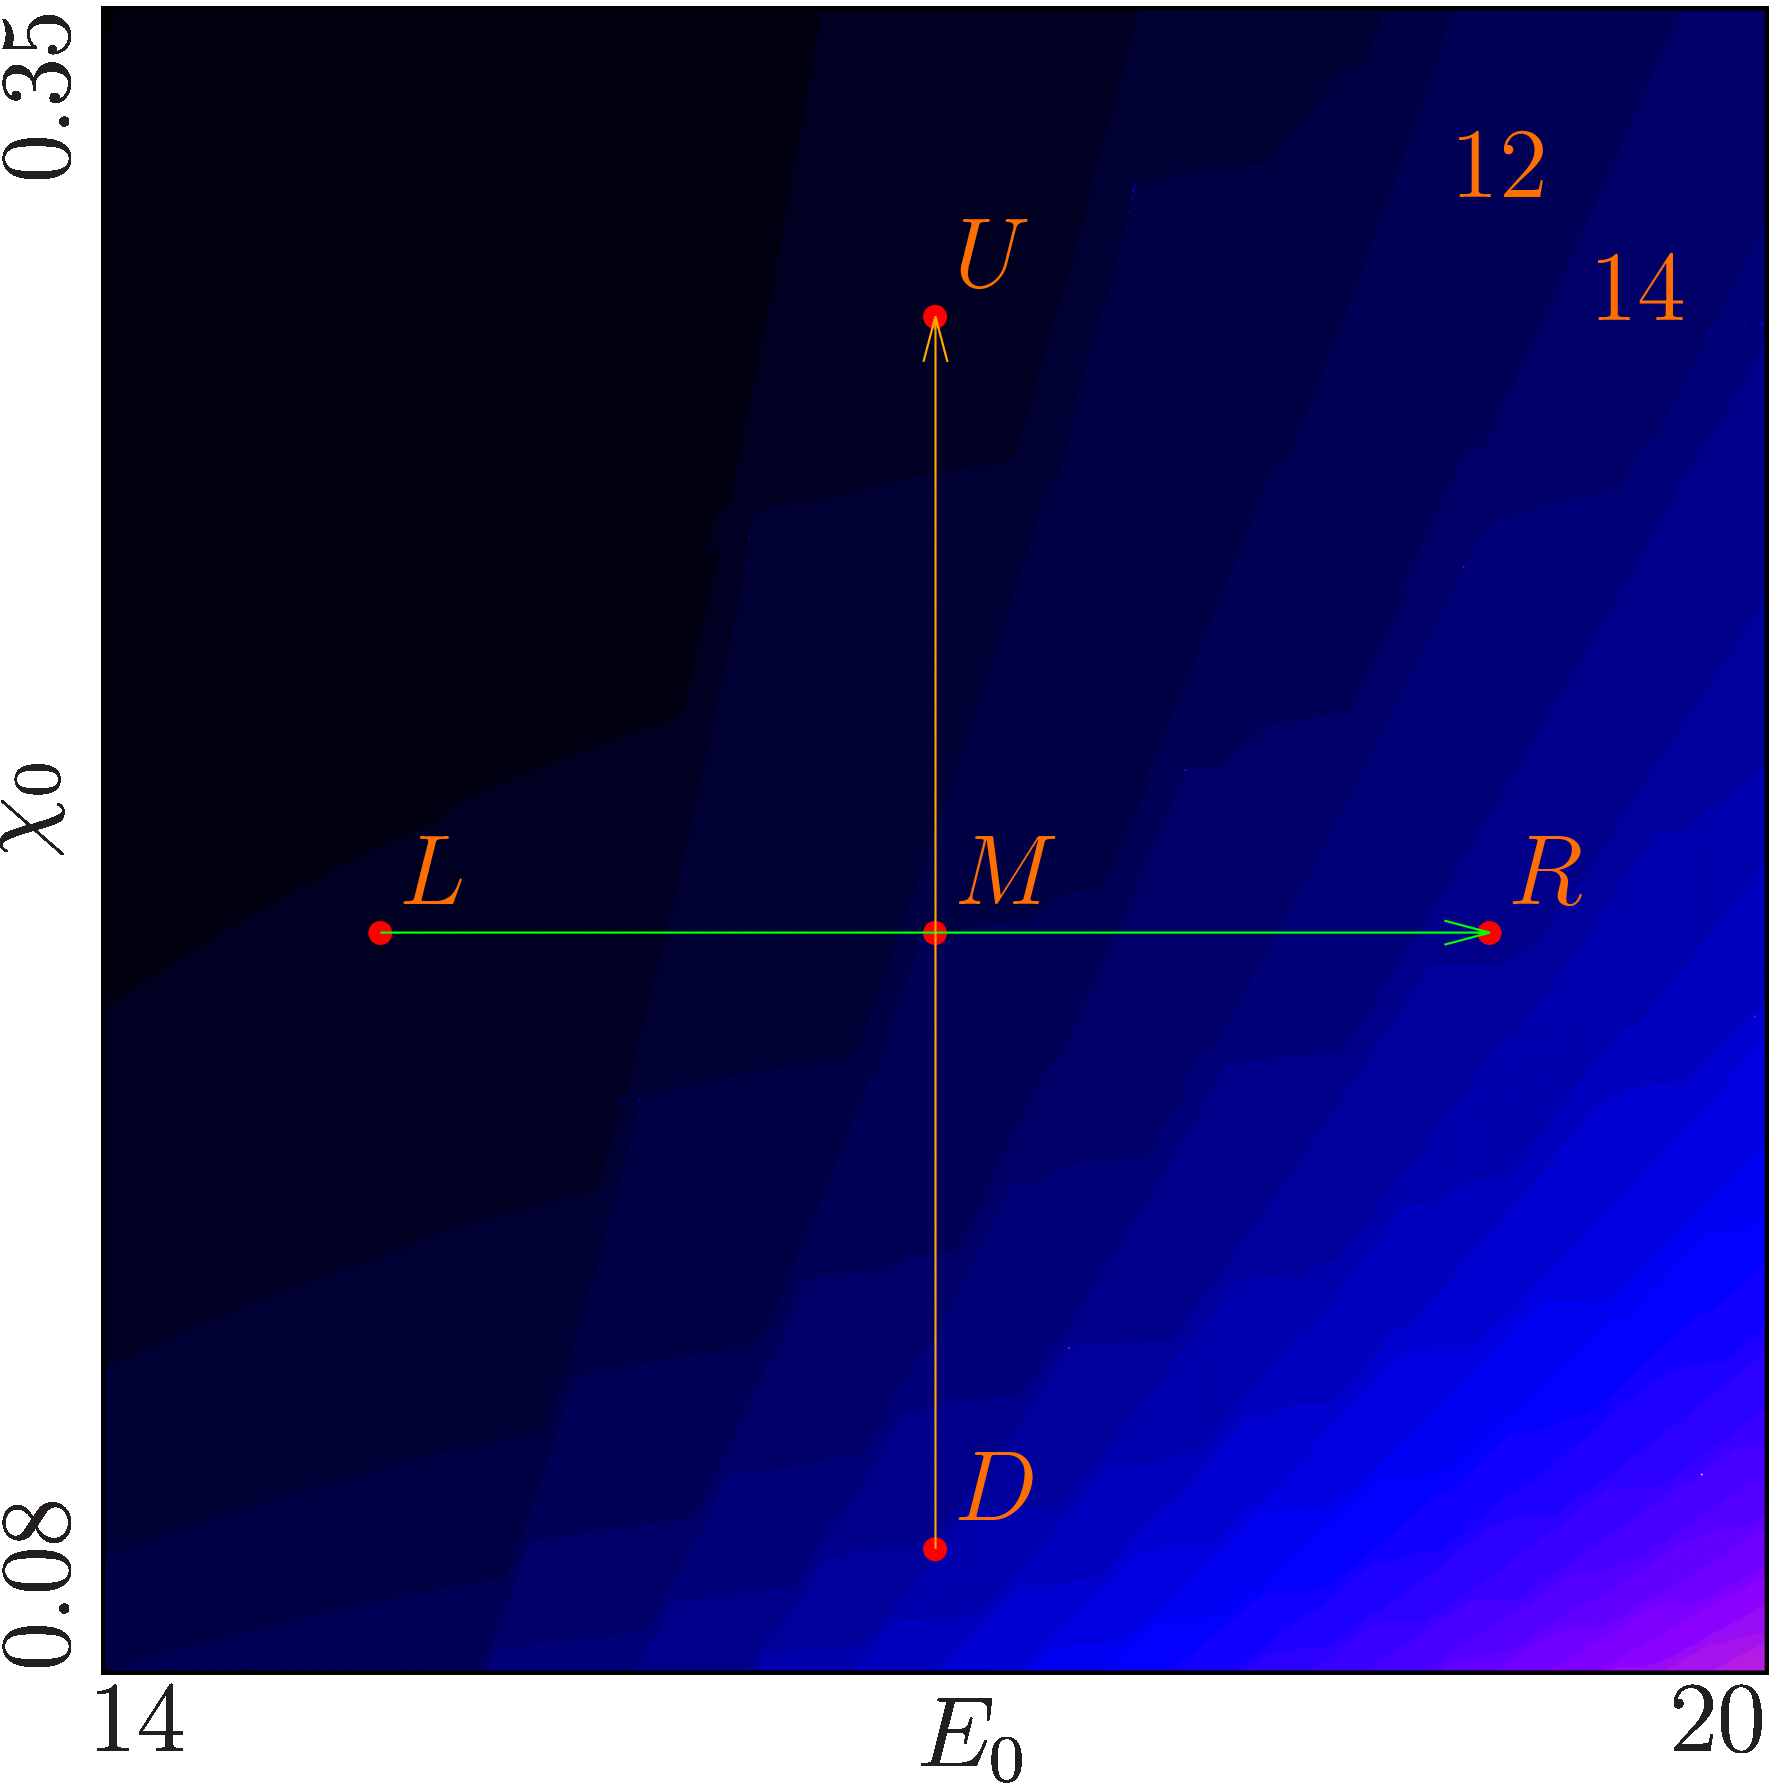
\includegraphics[width=0.4\textwidth]{../Figures/5/5.3/result.png}
	\caption[The parameter ranges examined to analyze the isolated effects of parameters on the original model function]{
		2D scan of the periods associated with parameter regions in the original model.
		The parameters $\beta = 1, f = 150, L = 4.2 \cdot 10^{-3}, R = 2, V_m = 5,$ and $\mu = 0.5$ are fixed.
		The parameters $E_0$ and $\chi_0$ are varied in the ranges $[14, 20]$ and $[0.08, 0.35]$.
		It illustrates the parameter ranges used to analyze the isolated effects of the parameters $E_0$ and $\chi_0$ on the original model function.
		The green arrow indicates the parameter range used to analyze the effects of the parameter $E_0$, while the orange arrow indicates the parameter range used to analyze the effects of the parameter $\chi_0$ on the original model function.
		The points $L, M, R, D,$ and $U$ mark the parameter values used for the cobweb diagrams in \Cref{fig:setup.char.evolution.single}.
	}
	\label{fig:setup.char.evolution.single.map}
\end{figure}

For the effects of the parameter $E_0$, $\chi_0 = 0.2$ is fixed and $E_0$ is varied in the parameter range $[15, 19]$.
This is marked as the green arrow in \Cref{fig:setup.char.evolution.single.map}.
As before, the model function is plotted at three parameter values in one figure.
The functions are visualized in \Cref{fig:setup.char.evolution.e0}.
$F^L$ is the model function with $E_0 = 15$, $F^M$ is the model function with $E_0 = 17$, and $F^R$ is the model function with $E_0 = 17$.
$\chi_0 = 0.2$ is the same for all functions $F^L, F^M,$ and $F^R$.
The parameter values are marked with the points $L, M,$ and $R$ in \Cref{fig:setup.char.evolution.single.map}.
One can see that they are all on the green arrow mentioned before.
The following changes can be observed.
\begin{enumerate}
	\item The values on the left sides of the branches $F_\B$ and $F_\D$ get smaller while the values on the right sides are not affected much.	\item The local minima of the branches $F_\B$ and $F_\D$ move left, and their values get smaller.
	\item The border between the branches $F_\A$ and $F_\B$ moves to the right.
	      The same is true for the border between the branches $F_\C$ and $F_\D$ because of the symmetry in the original model.
	\item The values at the right borders of branches $F_\A$ and $F_\C$ get larger. This is caused by the border between branches $F_\A$ and $F_B$ moving to the right.
\end{enumerate}

For the effects of the parameter $\chi_0$, $E_0 = 17$ is fixed and $\chi_0$ is varied in the parameter range $[0.125, 0.3]$.
This parameter range is marked with an orange arrow in \Cref{fig:setup.char.evolution.single.map}.
Again, the model function is plotted at three parameter values in one figure.
The functions are visualized in \Cref{fig:setup.char.evolution.hi}.
$F^D$ is the model function with $\chi_0 = 0.1$, $F^M$ is the model function with $\chi_0 = 0.2$, and $F^U$ is the model function with $\chi_0 = 0.3$.
$E_0 = 15$ is the same for all functions $F^D, F^M,$ and $F^U$.
The parameter values are marked with the points $D, M,$ and $U$ in \Cref{fig:setup.char.evolution.single.map}.
One can see that they are all on the orange arrow mentioned before.
The following pronounced changes can be observed.
\begin{enumerate}
	\item The values of the whole branches $F_\A$ and $F_\C$ get larger.
	\item The border between the branches $F_\A$ and $F_\B$ moves to the left.
	      The same is true for the border between the branches $F_\C$ and $F_\D$.
\end{enumerate}
Two other smaller changes that can be observed are the following.
\begin{enumerate}
	\item The values on the right sides of the branches $F_\B$ and $F_\D$ get larger.
	      This includes the values of the local minima on these branches.
	\item The border between the branches $F_\B$ and $F_\C$ moves to the left.
	      The same is true for the border between the branches $F_\D$ and $F_\A$.
\end{enumerate}

\begin{figure}
	\centering
	\subfloat[$E_0$]{
		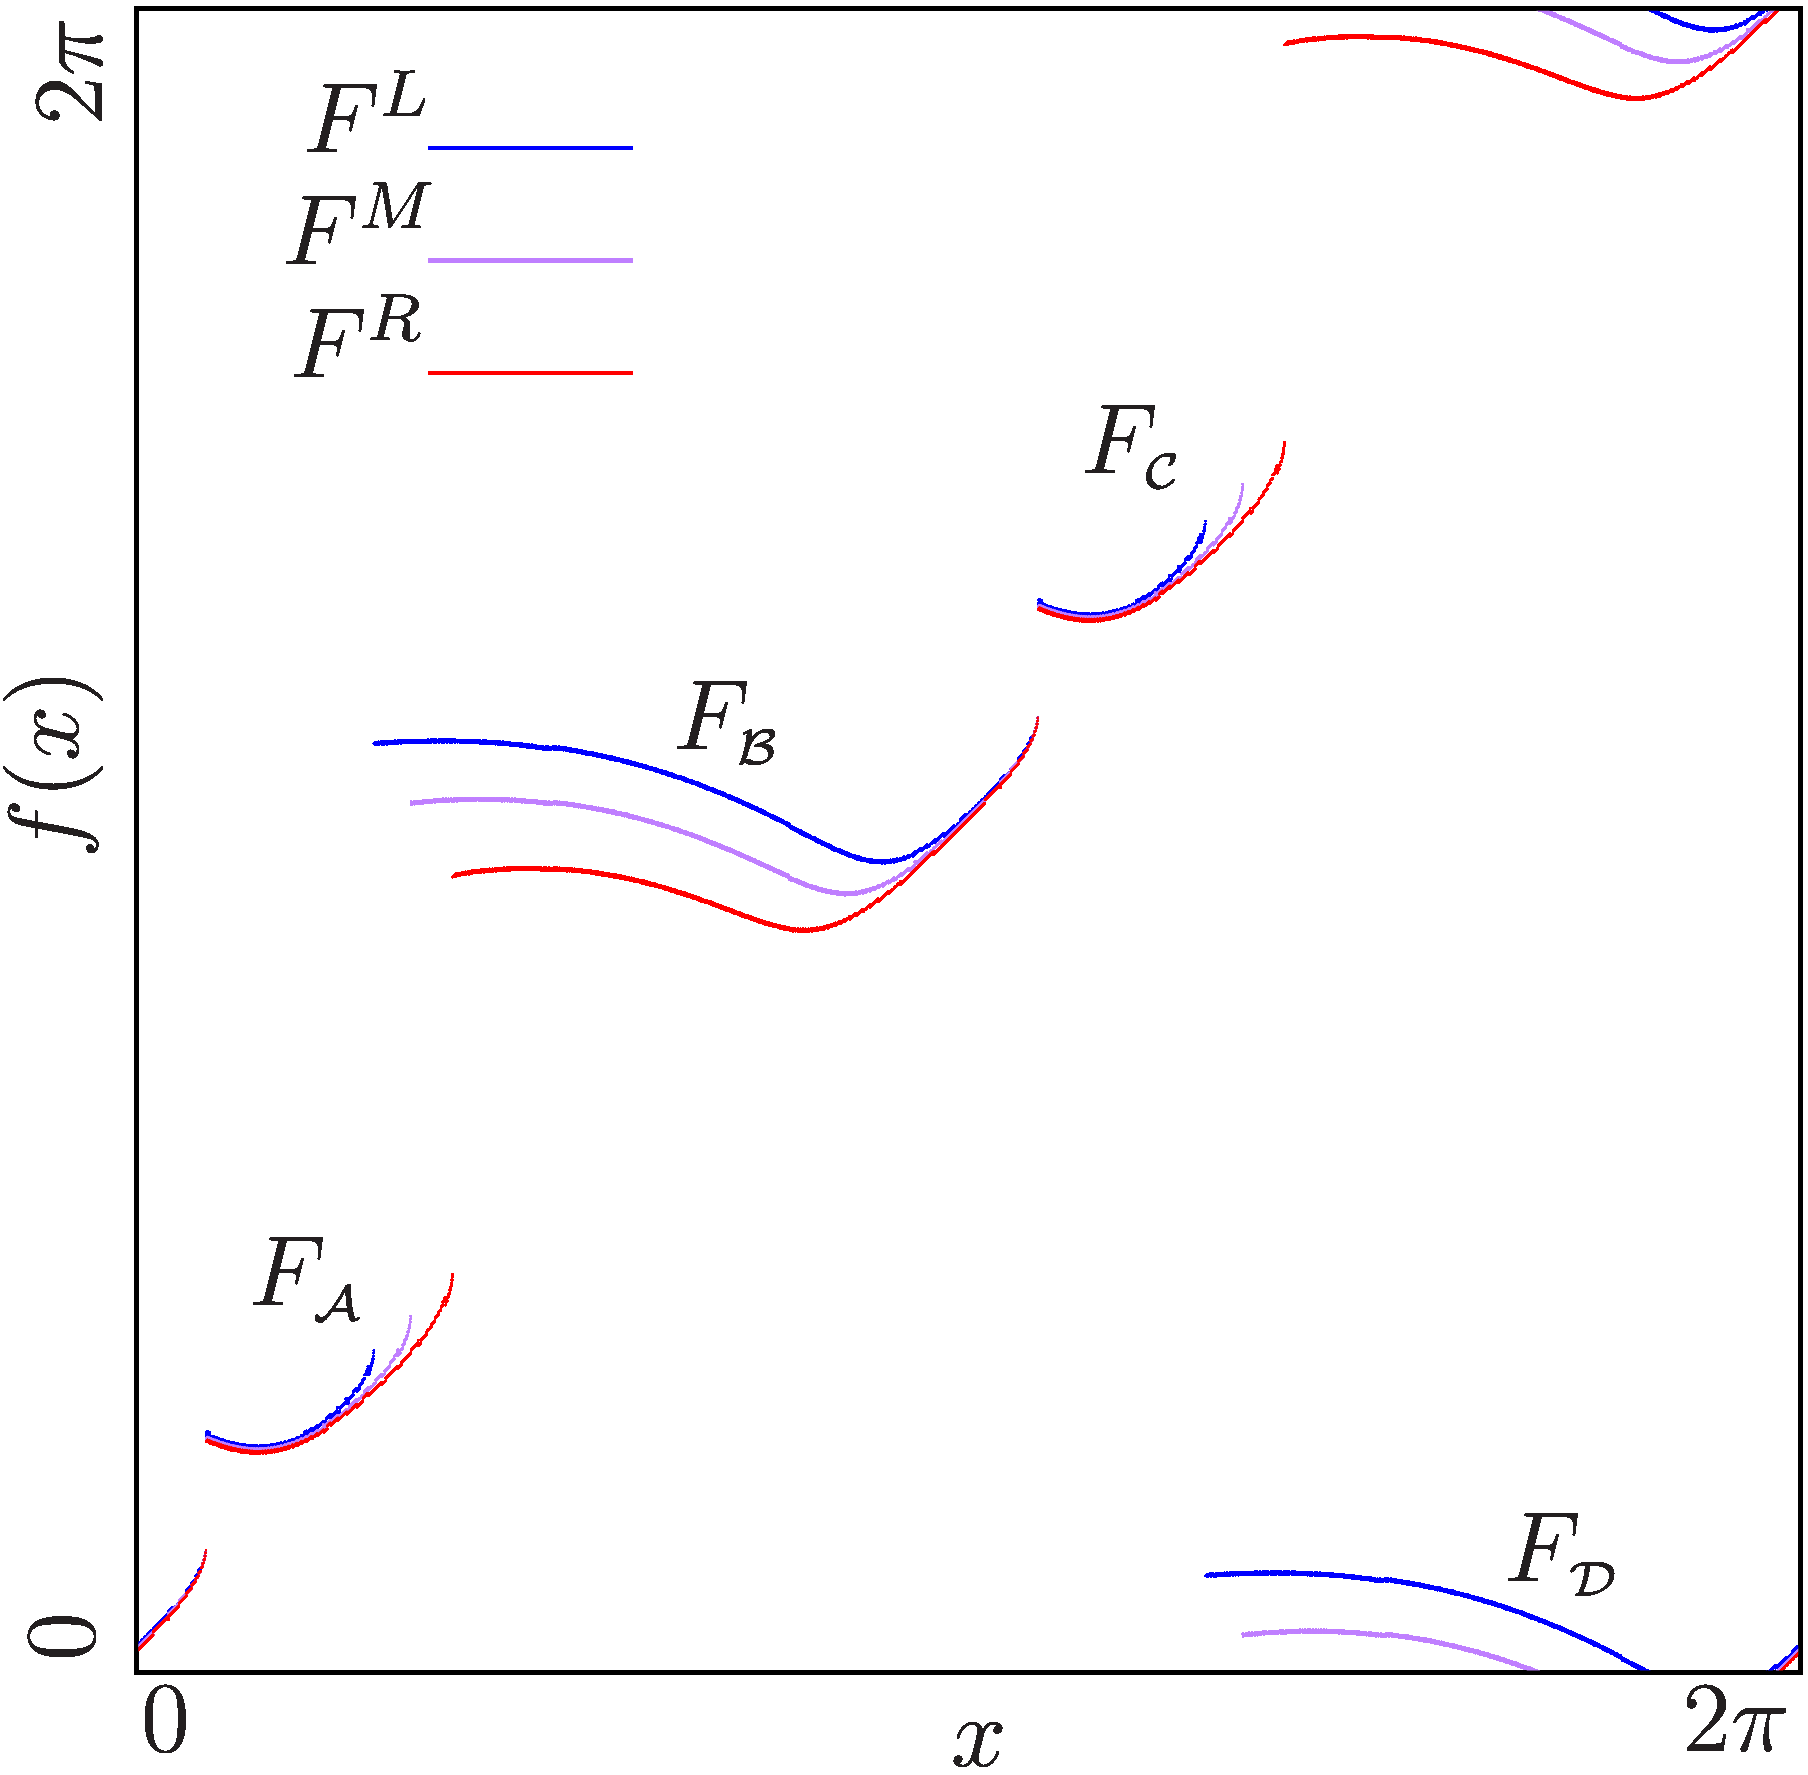
\includegraphics[width=.4 \textwidth]{../Figures/5/5.4a/illustration.png}
		\label{fig:setup.char.evolution.e0}
	}
	\subfloat[$\chi_0$]{
		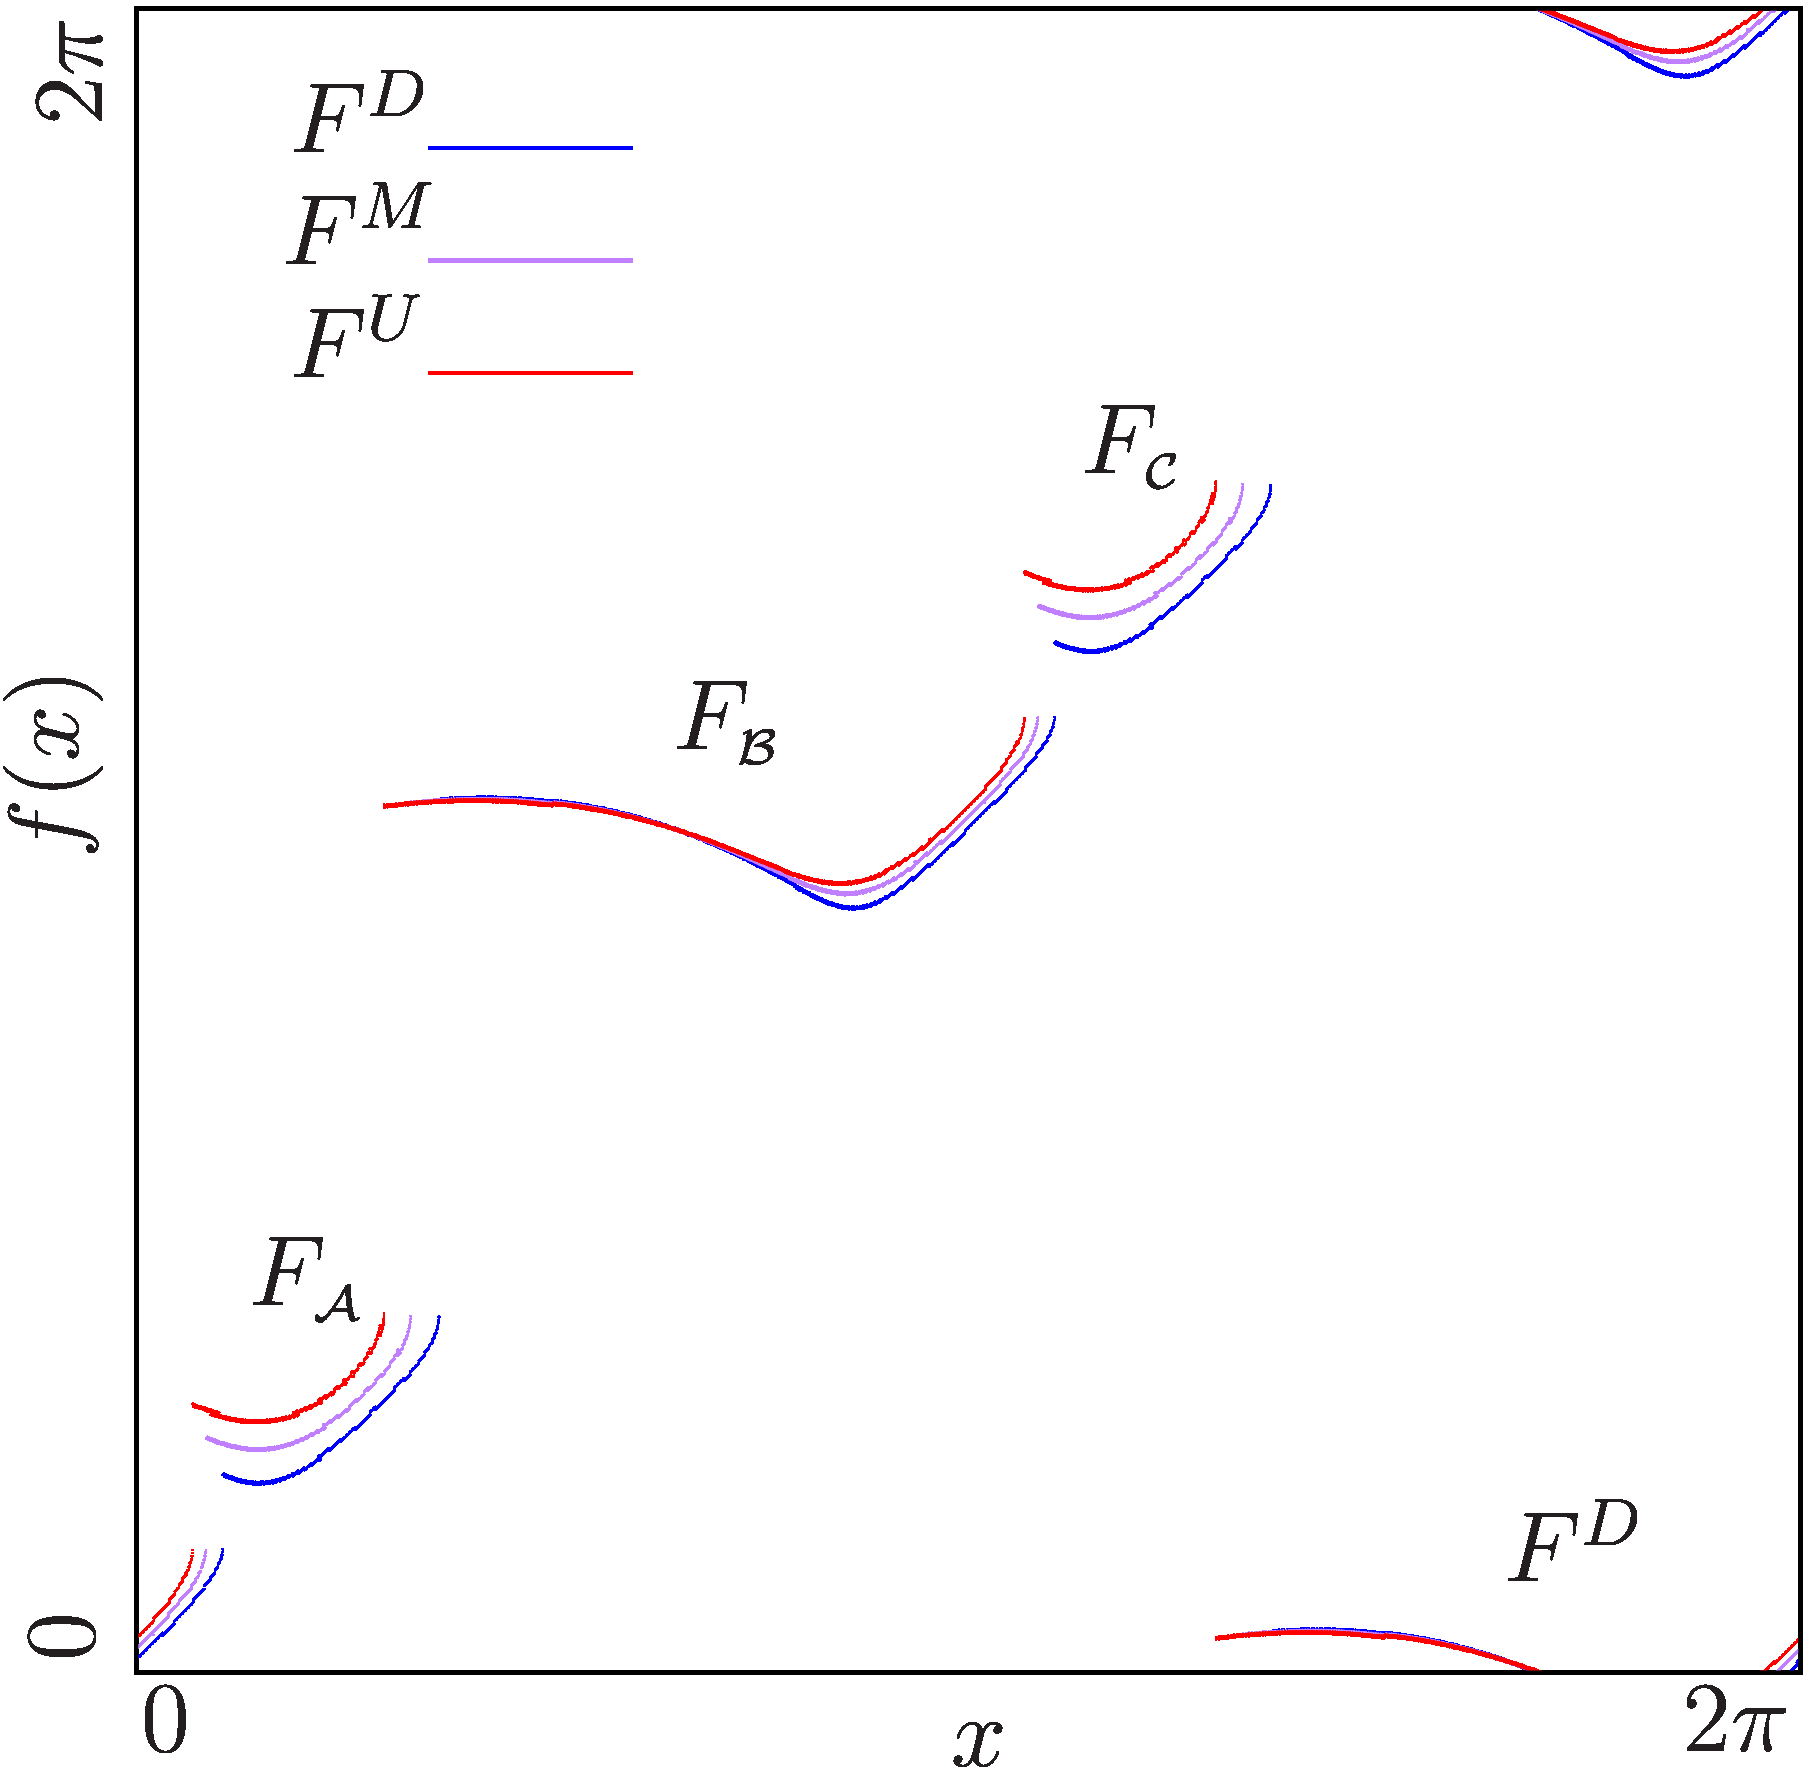
\includegraphics[width=.4 \textwidth]{../Figures/5/5.4b/illustration.png}
		\label{fig:setup.char.evolution.hi}
	}
	\caption[The isolated effects of the parameters on the original model function]{
		The isolated effects of the parameters $E_0$ and $\chi_0$ on the original model function.
		The parameter values used for plotting the functions are marked with points in \Cref{fig:setup.char.evolution.single.map}.
		(a) shows the evolution of the shape of the model function for different parameter values of $E_0$ while $\chi_0 = 0.2$ is fixed.
		The function $F^L$ is the model function with the parameter values at the point $L$ where $E_0 = 15$,
		$F^M$ is at the point $M$ where $E_0 = 17$,
		and $F^R$ is at the point $R$ where $E_0 = 19$.
		(b) shows the evolution of the shape of the model function for different parameter values of $\chi_0$ while $E_0 = 17$ is fixed.
		The function $F^D$ is the model function with the parameter values at the point $D$ where $\chi_0 = 0.1$,
		$F^M$ is at the point $M$ where $\chi_0 = 0.2$,
		and $F^U$ is at the point $U$ where $\chi_0 = 0.3$.
	}
	\label{fig:setup.char.evolution.single}
\end{figure}

\subsection{Decomposition of Combined Effects}
\label{sec:yunus.param.effects.decomposition}

This section considers the decomposition of the combined parameter effects listed in \Cref{sec:setup.char.paramfx.combined} into the effects of the isolated parameter effects listed in \Cref{sec:setup.char.paramfx.individual} and traces each effect back to its cause.
This is important, because some of the isolated parameter effects cancel out when the parameters are both varied as we will see later in this section.
For this, this section introduces a notation for the effects.
The effect of the values on the left side of a branch changing is denoted $\AL$, for the right side it is $\AR$, and for the whole branch it is $\AW$
The subscript indicates, which branch the change affects, and the superscript indicates, whether the values get larger $+$ or smaller $-$.
The effect of changing a local minimum is denoted as $\AMi$.
The meaning of the subscript stays the same as above, but the superscript also can include $L$ for movement to the left and $R$ for movement to the right.
Finally, the effect of moving borders is denoted as $\AB$.
The subscript now includes the two symbols of branches to which the border belongs and the superscript now has only $L$ or $R$.
For brevity, one does not write redundant branch names, so changes happening to branch $F_\A$ are also happening to branch $F_\C$.
For borders, changes to the border between branches $F_\A$ and $F_\B$ are also happening to the border between branches $F_\C$ and $F_\D$ and so on.

\Cref{table:setup.char.paramfx} lists all observed effects along the chains of parameter regions associated with cycles of the same period and their decomposition into effects of the single parameters.
The first part of the table includes all major changes observed in \Cref{sec:setup.char.paramfx.combined}.
The second part includes the minor change one can observe of the borders between the branches $f_\B$ and $f_\C$ moving to the left.
The second part also includes the changes observed in \Cref{sec:setup.char.paramfx.individual} that cancel out.
From this table we can see that $E_0$ causes the effects on the branches $F_\B$ and $F_\D$, while $\chi_0$ causes the changes to the branches $F_\A$ and $F_\C$, as well as the minor movement of the borders between the branches $F_\B$ and $F_\C$.
Note again that the change to the border of branches $F_\B$ and $F_\C$ also applies for the border between branches $F_\D$ and $F_\A$.

% table in next section for better layout



\todo{Figure out, which ones to keep}

%\section{Piecewise Linear Model}

The first model, we examined, is a simple piecewise linear function with four discontinuities.
Its discontinuities are at $0, \frac{\pi}{2}, \pi,$ and $\frac{3 \pi}{2}$.
\Cref{equ:pcw.lin.sympi} causes the discontinuities at $0$ and $\pi$ and also the symmetry $f(x + \pi) \equiv f(x) + \pi \mod 2 \pi$.

\begin{align}
    f(x) & = g(x) \mod 2 \pi \label{equ:pcw.lin.f} \\
    g(x) & = \begin{cases}
                 h(x)       & \text{ if } r(x) < \pi \\
                 h(x) + \pi & \text{ else}
             \end{cases} \label{equ:pcw.lin.sympi}
\end{align}

Each arm then is governed by \Cref{equ:pcw.lin.discpihalves}.
It causes the discontinuities at $\frac{\pi}{2}$ and $\frac{3 \pi}{2}$ and also shows the linear nature of the function.
Both parameters $\alpha$ and $\beta$ act here.
$\alpha$ is the slope of the arms and $\beta$ is the offset of the first and third arms.
Examples of how the function looks at different parameter values can be seen in the cobweb diagrams in \Cref{fig:pcw.lin.CobwebA-C}.

\begin{align}
    h(x) & = \begin{cases}
                 \alpha \cdot t(x) + \beta                      & \text{ if } s(x) < \frac{\pi}{2} \\
                 \alpha \cdot t(x) - \alpha \cdot \frac{\pi}{2} & \text{ else}
             \end{cases} \label{equ:pcw.lin.discpihalves}
\end{align}

\Cref{equ:pcw.lin.r,equ:pcw.lin.s} are used to make the above more readable.
They give the modulus of $x$ and some multiple of $\pi$.

\begin{align}
    r(x) & = x \mod 2 \pi \label{equ:pcw.lin.r} \\
    s(x) & = x \mod \pi \label{equ:pcw.lin.s}
\end{align}





\Cref{fig:pcw.lin.2d} shows a bifurcation diagram of the model described above.
The parameter $\beta$ is varied on the interval $[0, 2 \pi]$, because the model will behave the same for $[0, 2 \pi] + k \cdot 2 \pi$.
This is because the result of the function will be taken modulo $2 \pi$ in \Cref{equ:pcw.lin.f}.
The parameter $\alpha$ is varied on the interval $[0, 1]$ because for $\alpha < 0$ nothing especially interesting happens and for $\alpha > 1$ the model shows no periodic behavior.

\begin{figure}
    \centering
    \includegraphics[width=0.7\textwidth]{10_Linear_mod2pi/2D_Period/result.png}
    \caption{2D Bifurcation Diagram of Piecewise Linear Model}
    \label{fig:pcw.lin.2d}
\end{figure}

The two red lines mark the locations of the following one-dimensional scans keeping the parameter $\alpha$ fixed at $0.5$.
\Cref{fig:pcw.lin.1D} shows the scan along the lower red line.
There one can see a period-adding structure.
\Cref{fig:pcw.lin.1DPlusPi} shows the scan along the other red line.
The whole thing is not a period-adding structure, but there is a period-adding structure on the left and on the right of the line in the middle.
Both these structures don't look like period-adding structures normally do.
The interval in the middle of each structure is not the biggest interval with a constant period, but rather some interval that's further to the middle of both structures.

\begin{figure}
    \centering
    \begin{subfigure}{0.4\textwidth}
        \centering
        \includegraphics[width=\textwidth]{10_Linear_mod2pi/1D_Period/result.png}
        \caption{$\beta \in [0.7, 1.7]$}
        \label{fig:pcw.lin.1D}
    \end{subfigure}
    \begin{subfigure}{0.4\textwidth}
        \centering
        \includegraphics[width=\textwidth]{10_Linear_mod2pi/1D_Period_PlusPi/result.png}
        \caption{$\beta \in [3.84, 4.84]$}
        \label{fig:pcw.lin.1DPlusPi}
    \end{subfigure}
    \caption{1D Scans of Piecewise Linear Model showing Periods}
\end{figure}

\Cref{fig:pcw.lin.CobwebA-C} shows a collection of cobwebs diagrams of the three points $P_A$ to $P_C$ marked in \Cref{fig:pcw.lin.1D}.
Note that in this period-doubling structure, all cycles exist in pairs.
At point $P_A$, there are two cycles of period 2 with the symbolic sequences $\A\B$ and $\C\D$ respectively.
When we make the parameter $\beta$ smaller, the cycles move toward the left of the arms.
\Cref{fig:pcw.lin.CobwebA} shows the cycles at the edge of the arms, shortly after that, the cycles collide with the border of the arms.

In the middle interval of \Cref{fig:pcw.lin.1D} with constant period 3, the cycles of $P_A$ are added with the fixed points of the left side.
This Farey-like-adding of cycles is common in period-adding structures~\cite{avrutin2019continuous}.
The fixed points are not shown here but are in the arms $\A$ and $\C$ respectively.
The resulting cycles are $\A^2\B$ and $\C^2\D$ and are shown in \Cref{fig:pcw.lin.CobwebB,fig:pcw.lin.CobwebC}.
These cobweb diagrams also make the movement of the cycles with decreasing parameter $\beta$, mentioned above, clear.
At $P_B$, $\beta$ is bigger and the cycles are at the right edge of the arms.
At $P_C$, the cycles are again at the left edge of the arms.

\begin{figure}
    \centering
    \begin{subfigure}{0.3\textwidth}
        \centering
        \includegraphics[width=\textwidth]{10_Linear_mod2pi/Cobweb_A/result.png}
        \caption{$P_A$}
        \label{fig:pcw.lin.CobwebA}
    \end{subfigure}
    \begin{subfigure}{0.3\textwidth}
        \centering
        \includegraphics[width=\textwidth]{10_Linear_mod2pi/Cobweb_B/result.png}
        \caption{$P_B$}
        \label{fig:pcw.lin.CobwebB}
    \end{subfigure}
    \begin{subfigure}{0.3\textwidth}
        \centering
        \includegraphics[width=\textwidth]{10_Linear_mod2pi/Cobweb_C/result.png}
        \caption{$P_C$}
        \label{fig:pcw.lin.CobwebC}
    \end{subfigure}
    \caption{Cobwebs for first 1D Scan}
    \label{fig:pcw.lin.CobwebA-C}
\end{figure}

\Cref{fig:pcw.lin.CobwebD-F} shows three cobwebs for different points of the second 1D scan in \Cref{fig:pcw.lin.1DPlusPi}.
You can see, that the cycles here do not follow Farey-like-adding like in the other 1D scan.
This is of course because the three cobwebs do not belong to one period adding structure.
The cycles are nonetheless interesting.
The two-cycle at $P_D$, shown in \Cref{fig:pcw.lin.CobwebD}, has the symbolic sequence $\A\C$.
It is on the right edge of the arms at this point and after colliding and skipping the period adding structure, two coexisting cycles appear, shown in \Cref{fig:pcw.lin.CobwebE}.
They have symbolic sequences $\A\D\C$ and $\A\C\B$ respectively.
It is safe to assume, that in the period adding structure between the two points, $P_D$ and $P_E$, the cycles follow Farrey-adding.

\Cref{fig:pcw.lin.CobwebF} shows the 4-cycle at the point $P_F$.
It has the symbolic sequence $\A\D\C\B$ and is at the left edge of the arms.
Lowering the parameter $\beta$ will cause the cycle to collide with the borders and this in turn will lead to the period adding structure we see in the 1D scan in \Cref{fig:pcw.lin.1DPlusPi}.
This period-adding structure will also follow the Farey-like-adding of this cycle and the 3-cycles at point $P_E$, shown in \Cref{fig:pcw.lin.CobwebE}.

\begin{figure}
    \centering
    \begin{subfigure}{0.3\textwidth}
        \centering
        \includegraphics[width=\textwidth]{10_Linear_mod2pi/Cobweb_D/result.png}
        \caption{$P_D$}
        \label{fig:pcw.lin.CobwebD}
    \end{subfigure}
    \begin{subfigure}{0.3\textwidth}
        \centering
        \includegraphics[width=\textwidth]{10_Linear_mod2pi/Cobweb_E/result.png}
        \caption{$P_E$}
        \label{fig:pcw.lin.CobwebE}
    \end{subfigure}
    \begin{subfigure}{0.3\textwidth}
        \centering
        \includegraphics[width=\textwidth]{10_Linear_mod2pi/Cobweb_F/result.png}
        \caption{$P_F$}
        \label{fig:pcw.lin.CobwebF}
    \end{subfigure}
    \caption{Cobwebs for second 1D Scan}
    \label{fig:pcw.lin.CobwebD-F}
\end{figure}


\section{Piecewise Quadratic Model}

In this section, we will examine the dynamics of a piecewise quadratic model.
Starting with a model with 4 branches and symmetry, like in \Cref{sec:og.full}.
After that, we will reduce the model to just two branches using symmetry.

\subsection{Full Model}

\todo{make mod generic}

The full model is the map $x \mapsto f(x) \mod 6$.
Where $f$ is given by the following collection of equations.
\begin{align}
    f(x) & = \begin{cases}
                 g(x)     & \text{if } r(x) < 3 \\
                 g(x) + 3 & \text{else}
             \end{cases} \label{equ:quad.full.f}                                    \\
    g(x) & = \begin{cases}
                 a_L \cdot s_L(x)^2 + b_L \cdot x + c_L & \text{if } s(x) < \frac{3}{2} \\
                 a_R \cdot s_R(x)^2 + b_R \cdot x + c_R & \text{else}
             \end{cases} \label{equ:quad.full.g}
\end{align}

\Cref{equ:quad.full.f} causes the disontinuity in the middle at $x = 3$.
It also makes sure, the symmetry $f(x + 3) \equiv f(x) + 3 \mod 6$ is true.
Each half of the model is then governed by \Cref{equ:quad.full.g}.
Here all the 6 parameters $a_L, a_R, b_L, b_R, c_L,$ and $c_R$ act.

\todo{describe offset by s and t}
\todo{split g into l and r needed later for fitting}

\Crefrange{equ:quad.full.s}{equ:quad.full.sr} provide adjusted values of x for either choosing between branches in both halves or substituting in the quadratic formulas of each branch.
\begin{subequations}
    \begin{align}
        s(x)   & = x \mod 3 \label{equ:quad.full.s}            \\
        s_L(x) & = s(x) - \frac{3}{4}                          \\
        s_R(x) & = s(x) - \frac{9}{4} \label{equ:quad.full.sr}
    \end{align}
\end{subequations}

\subsection{Variation of Single Parameters}

We start by examining the behavior of the quadratic model under variations of single parameters like $a_L, a_R, b_L, b_R, c_L,$ and $c_R$.

\subsubsection{Fixing $a_L = a_R = 1, b_L = b_R = 0$}

\Cref{fig:quadratic.full.2d.full} shows a 2D-scan of the periods of the stable cycles.
The parameters $a_L = a_R = 1$ and $b_L = b_R = 0$ are fixed and the parameters $c_L$ and $c_R$ are varied.
Both are varied within the range $[0, 6]$ because beyond that the diagram just repeats infinitely.
The structure in the middle left is enhanced and depicted in \Cref{fig:quadratic.full.2d.z1}.

\begin{figure}
    \centering
    \begin{subfigure}{0.4\textwidth}
        \centering
        \includegraphics[width=\textwidth]{21_Quadratic_mod6/2D_Period_Full/result.png}
        \caption{Full}
        \label{fig:quadratic.full.2d.full}
    \end{subfigure}
    \begin{subfigure}{0.4\textwidth}
        \centering
        \includegraphics[width=\textwidth]{21_Quadratic_mod6/2D_Period_Zoomed1/result.png}
        \caption{Zoomed}
        \label{fig:quadratic.full.2d.z1}
    \end{subfigure}
    \caption{2D Scan of Full Quadratic Model}
\end{figure}

A phenomenon like in the original model could not be found here.
But something very similar happens on the border of these wings.
\Cref{fig:quad.full.Cobwebs} shows the cobwebs along the line marked in \Cref{fig:quadratic.full.2d.z1}.
Before the border, there is one stable cycle with period 8.
This cycle is depicted in \Cref{fig:quad.full.CobwebA} and its symbolic sequence is $\A^3B\C^3\D$.
At the border, there is an area where two cycles coexist.
You cannot see this in the 2D scans above, since it only ever picks up on one cycle.
\Cref{fig:quad.full.CobwebB} shows the coexisting cycles at this border.
In contrast to the original model, the cycle that existed before in \Cref{fig:quad.full.CobwebA}, still exists alongside the new cycle with period 6.
The symbolic sequence of the new cycle is $\A^2\B\C^2\D$.

This is different from the dynamics in the original model in two ways.
First, the cycles before and after the area of coexistence have different periods.
And second, the cycles existing outside the area of coexistence still exist inside the area of coexistence.
In the original model, the cycles existing outside the area of coexistence would disappear at the border and new cycles would emerge inside this area.

\begin{figure}
    \centering
    \begin{subfigure}{0.3\textwidth}
        \centering
        \includegraphics[width=\textwidth]{21_Quadratic_mod6/Cobweb_A/result.png}
        \caption{Before border}
        \label{fig:quad.full.CobwebA}
    \end{subfigure}
    \begin{subfigure}{0.3\textwidth}
        \centering
        \includegraphics[width=\textwidth]{21_Quadratic_mod6/Cobweb_B/result.png}
        \caption{At border}
        \label{fig:quad.full.CobwebB}
    \end{subfigure}
    \begin{subfigure}{0.3\textwidth}
        \centering
        \includegraphics[width=\textwidth]{21_Quadratic_mod6/Cobweb_C/result.png}
        \caption{After border}
        \label{fig:quad.full.CobwebC}
    \end{subfigure}
    \caption{Cobwebs along marked line}
    \label{fig:quad.full.Cobwebs}
\end{figure}

\subsubsection{Fixing $a_L = a_R = b_L = b_R = 1$}

If you compare the functions in the cobwebs \Crefrange{fig:quad.full.CobwebA}{fig:quad.full.CobwebB} to the functions of the original model in \Crefrange{fig:yunus.2pi.CobwebA2}{fig:yunus.2pi.CobwebD2} one can see some differences.
One is, that the right end of the branches $\B$ and $\D$ is higher than the left part.
To get our model to look a little more like the original model, we now skew the branches by fixing also $b_L = b_R = 1$

The 2D scan for the periods when varying $c_L$ and $c_R$ now looks different.
\Cref{fig:quadratic.full.skew.2d.full} shows the full scan, while \Cref{fig:quadratic.full.skew.2d.z1} shows an enhanced version of it, depicting the artefact in the middle of the left half of the full scan.
\Cref{fig:quadratic.full.skew.2d.c} shows an enhanced version of the 2D scans depicting an interesting area where some cobwebs were taken.
The area is where a wing with stable cycles of period 12 connects with a wing of the same period.
There is a red line in the figure, it marks where the cobwebs are taken.

\begin{figure}
    \centering
    \begin{subfigure}{0.4\textwidth}
        \centering
        \includegraphics[width=\textwidth]{21_Quadratic_mod6/Skew/2D_Period_SFull/result.png}
        \caption{Full}
        \label{fig:quadratic.full.skew.2d.full}
    \end{subfigure}
    \begin{subfigure}{0.4\textwidth}
        \centering
        \includegraphics[width=\textwidth]{21_Quadratic_mod6/Skew/2D_Period_SZoomed1/result.png}
        \caption{Zoomed}
        \label{fig:quadratic.full.skew.2d.z1}
    \end{subfigure}
    \caption{2D Scan of Full Skewed Quadratic Model}
\end{figure}

\begin{figure}
    \centering
    \includegraphics[width=0.4\textwidth]{21_Quadratic_mod6/Skew/2D_Period_SC/result.png}
    \caption{2D Scan of Interesting Area of Full Skeqed Quadratic Model}
    \label{fig:quadratic.full.skew.2d.c}
\end{figure}

\Cref{fig:quad.full.skew.c.Cobwebs} shows all the cobwebs taken along the red line in \Cref{fig:quadratic.full.skew.2d.c}.
The first one, \Cref{fig:quad.full.skew.c.CobwebA}, shows a cycle with period 12.
Its symbolic sequence is $\A^4\B^2\C^4\D^2$.
The last cobweb, \Cref{fig:quad.full.skew.c.CobwebC}, also shows a 12-cycle, this time with symbolic sequence $\A^3\B^3\C^3\D^3$.
Here, one point from branches $\A$ and $\C$ moved to branches $\B$ and $\D$, the same thing that happened in the original model.
And in the middle, there is also coexistence of two 12-cycles.
This is depicted in \Cref{fig:quad.full.skew.c.CobwebB}.
The difference is, that in this case, the symbolic sequences of the two coexisting 12-cycles are $\Cycle{\A^4\B^2\C^4\D^4}$ and $\Cycle{\A^3\B^3\C^3\D^3}$.
This is different from the original model because there the symbolic sequences were $\A^3\B^3\C^2\D^4$ and $\A^2\B^4\C^3\D^3$, which were different from both 12-cycles existing outside the area of coexistence.
Here, the 12-cycles existing outside the coexistence area continue to exist inside it.

\begin{figure}
    \centering
    \begin{subfigure}{0.3\textwidth}
        \centering
        \includegraphics[width=\textwidth]{21_Quadratic_mod6/Skew/Cobweb_SC/result_A.png}
        \caption{Before border}
        \label{fig:quad.full.skew.c.CobwebA}
    \end{subfigure}
    \begin{subfigure}{0.3\textwidth}
        \centering
        \includegraphics[width=\textwidth]{21_Quadratic_mod6/Skew/Cobweb_SC/result_B.png}
        \caption{At border}
        \label{fig:quad.full.skew.c.CobwebB}
    \end{subfigure}
    \begin{subfigure}{0.3\textwidth}
        \centering
        \includegraphics[width=\textwidth]{21_Quadratic_mod6/Skew/Cobweb_SC/result_C.png}
        \caption{After border}
        \label{fig:quad.full.skew.c.CobwebC}
    \end{subfigure}
    \caption{Cobwebs along marked line}
    \label{fig:quad.full.skew.c.Cobwebs}
\end{figure}

\subsubsection{Fixing $a_L = a_R = b_L = 1, c_R = 2.3$}

To better mimic the behavior of the original model function, we now fix the parameters $a_L, a_R, b_L,$ and $c_R$.
Fixing $a_L$ and $b_L$ and varying $c_L$ in the range $[0.8, 1.4]$ will cause the branches $\A$ and $\C$ to move upwards, just as we observed in the original model in \Cref{sec:og.param.effects}.
To get the left part of branches $\B$ and $\D$ to move downwards while also moving the local minima of those branches to the lower left, we vary $b_R$ in the range $[0, 2]$.
\Cref{fig:quadratic.full.cLbR.2d.full} shows a 2D scan of the periods in this model.


\begin{figure}
    \centering
    \includegraphics[width=0.6\textwidth]{21_Quadratic_mod6/TestingDifferentParameters/cLbR/2D_Period_cLbR/result.png}
    \caption{2D Scan of Quadratic Model Imitating the Original Model}
    \label{fig:quadratic.full.cLbR.2d.full}
\end{figure}

\Cref{fig:quad.full.cLbR.Cobwebs} shows cobwebs along the red line in \Cref{fig:quadratic.full.cLbR.2d.full}.
You can see, that the 14-cycle that existed at the beginning in \Cref{fig:quad.full.cLbR.CobwebA} with symbolic sequence $\A^3\B^4\C^3\D^4$ still exists at the end in \Cref{fig:quad.full.cLbR.CobwebC}.
In \Cref{fig:quad.full.cLbR.CobwebB} one can also see another 14-cycle coexisting.
It has the symbolic sequence $\A^2\B^5\C^2\D^5$.
This is different from the phenomenon, we are searching for.
The reason for this coexistence is, that the arm of the wing crosses this area of period 14.
You can see the arm above the right end of the red line passing through the arm of the area we are examining.

\begin{figure}
    \centering
    \begin{subfigure}{0.3\textwidth}
        \centering
        \includegraphics[width=\textwidth]{21_Quadratic_mod6/TestingDifferentParameters/cLbR/Cobweb_cLbR/result_A.png}
        \caption{Before border}
        \label{fig:quad.full.cLbR.CobwebA}
    \end{subfigure}
    \begin{subfigure}{0.3\textwidth}
        \centering
        \includegraphics[width=\textwidth]{21_Quadratic_mod6/TestingDifferentParameters/cLbR/Cobweb_cLbR/result_B.png}
        \caption{At border}
        \label{fig:quad.full.cLbR.CobwebB}
    \end{subfigure}
    \begin{subfigure}{0.3\textwidth}
        \centering
        \includegraphics[width=\textwidth]{21_Quadratic_mod6/TestingDifferentParameters/cLbR/Cobweb_cLbR/result_C.png}
        \caption{After border}
        \label{fig:quad.full.cLbR.CobwebC}
    \end{subfigure}
    \caption{Cobwebs along marked line}
    \label{fig:quad.full.cLbR.Cobwebs}
\end{figure}

\subsubsection{Fixing $a_L = a_R = 1, c_L = 1.03, c_R = 2.5$}

Since varying $c_L$ in the positive direction lifts both sides of branches $\A$ and $\C$ and in the original model only the left side moves upwards, we now try to fix $c_L$ and instead vary $b_L$.
\Cref{fig:quadratic.full.bLbR.2d.full} shows a 2D scan of the behavior of cycles in this model under variation of $b_L$ and $b_R$.
\Cref{fig:quadratic.full.bLbR.2d.z} shows a zoomed-in version of that 2D scan with three points, where cobwebs are made.
In the areas containing the three points, something similar happens, to what is happening in the original model.

\begin{figure}
    \centering
    \begin{subfigure}{0.4\textwidth}
        \centering
        \includegraphics[width=\textwidth]{21_Quadratic_mod6/TestingDifferentParameters/bLbR/2D_Period_bLbR/result.png}
        \caption{Full}
        \label{fig:quadratic.full.bLbR.2d.full}
    \end{subfigure}
    \begin{subfigure}{0.4\textwidth}
        \centering
        \includegraphics[width=\textwidth]{21_Quadratic_mod6/TestingDifferentParameters/bLbR/2D_Period_bLbR_Zoomed/result.png}
        \caption{Zoomed}
        \label{fig:quadratic.full.bLbR.2d.z}
    \end{subfigure}
    \caption{2D Scan of Model Imitating the Original model \todo{choose better caption, labels different color}}
\end{figure}

The cobwebs are side by side in \Cref{fig:quad.full.bLbR.Cobwebs}.
The first cycle at point $A$, depicted in \Cref{fig:quad.full.bLbR.CobwebA}, has period 18 and its symbolic sequence is $\A^4\B^4\C^4\D^4$.
The cycle at point $C$, depicted in \Cref{fig:quad.full.bLbR.CobwebC}, has period 12 and its symbolic sequence is $\A^3\B^3\C^3\D^3$.
Thus far, what happens here has nothing to do with our original model, since the periods are different.
But in the middle, something interesting is happening.
At point $B$, two cycles are coexisting.
Note that the point was chosen lower to better illustrate the following observations, the same thing is happening in the whole area of this color.
The first one has period 14 and its symbolic sequence is $\A^4\B^4\C^3\D^3$.
And the other one also has period 14 and its symbolic sequence is $\A^3\B^3\C^4\D^4$.
This is similar to the original model because there the coexisting cycles also behaved like the one cycle on the left half of the model and like the other cycle on the right half of the model.

\begin{figure}
    \centering
    \begin{subfigure}{0.3\textwidth}
        \centering
        \includegraphics[width=\textwidth]{21_Quadratic_mod6/TestingDifferentParameters/bLbR/Cobweb_bLbR_A/result.png}
        \caption{Point A}
        \label{fig:quad.full.bLbR.CobwebA}
    \end{subfigure}
    \begin{subfigure}{0.3\textwidth}
        \centering
        \includegraphics[width=\textwidth]{21_Quadratic_mod6/TestingDifferentParameters/bLbR/Cobweb_bLbR_B/result.png}
        \caption{Point B}
        \label{fig:quad.full.bLbR.CobwebB}
    \end{subfigure}
    \begin{subfigure}{0.3\textwidth}
        \centering
        \includegraphics[width=\textwidth]{21_Quadratic_mod6/TestingDifferentParameters/bLbR/Cobweb_bLbR_C/result.png}
        \caption{Point C}
        \label{fig:quad.full.bLbR.CobwebC}
    \end{subfigure}
    \caption{Cobwebs at marked points}
    \label{fig:quad.full.bLbR.Cobwebs}
\end{figure}

\subsection{Combining Parameter}

Thus far, we have not seen type B regions, that are not caused by overlapping type A regions.
We now want to change multiple parameters at the same time to imitate the function of the original model better.
For this, we introduce new parameters, $p_x$ and $p_y$, and define the actual model parameters dependent on those two.

\subsubsection{Defining $a_R = 1 + p_x$, $b_R = 2 \cdot px$, and $c_L = p_y$}

\todo{full scan}

\begin{figure}
    \centering
    \begin{subfigure}{0.4\textwidth}
        \centering
        \includegraphics[width=\textwidth]{21_000_Quadratic_1aR2bR_cL/LU/2D_Period_LU/result.png}
        \caption{Periods}
        \label{fig:quadratic.full.1aR2bR_cL.2d.1}
    \end{subfigure}
    \begin{subfigure}{0.4\textwidth}
        \centering
        \includegraphics[width=\textwidth]{21_000_Quadratic_1aR2bR_cL/LU/2D_Regions_LU/result.png}
        \caption{Period Regions}
        \label{fig:quadratic.regions.1aR2bR_cL.2d.1}
    \end{subfigure}
    \caption{2D Scans of First Marked Region}
\end{figure}

\todo{some cobwebs}

\todo{lower regions nothing to be found}


\subsubsection{Defining $a_R = 1 + 2 \cdot p_x$, $b_R = px$, and $c_L = p_y$}

This definition of $a_R$ and $b_R$ is similar to before, but now $p_x$ has double the effect on $a_R$ and half the effect on $b_R$.
It was created by accident since it does not imitate the original model as nicely as before.
\Cref{fig:quadratic.full.2aR1bR_cL.2d.full} shows the 2D scan of the different periods.
Regions we will have a closer look at, are marked with red rectangles.

\begin{figure}
    \centering
    \includegraphics[width=0.6\textwidth]{21_010_Quadratic_2aR1bR_cL/2D_Period_Selected/result.png}
    \caption{2D Scan of Periods of Quadratic Model with ...}
    \label{fig:quadratic.full.2aR1bR_cL.2d.full}
\end{figure}

The first enhanced region, shown in \Cref{fig:quadratic.full.2aR1bR_cL.2d.1}, has two areas with stable cycles of period 6 that overlap.
\Cref{fig:quadratic.regions.2aR1bR_cL.2d.1} shows the borders of the two regions.
It was created by halving the model and scanning for the borders of regions of different periods.
We will see that the bottom area is a type B area, and therefore the period in the halved model is double the period in the full model.

\begin{figure}
    \centering
    \begin{subfigure}{0.4\textwidth}
        \centering
        \includegraphics[width=\textwidth]{21_010_Quadratic_2aR1bR_cL/P6/2D_Period_P6/result.png}
        \caption{Periods}
        \label{fig:quadratic.full.2aR1bR_cL.2d.1}
    \end{subfigure}
    \begin{subfigure}{0.4\textwidth}
        \centering
        \includegraphics[width=\textwidth]{21_010_Quadratic_2aR1bR_cL/P6/2D_Regions_P6/result.png}
        \caption{Period Regions}
        \label{fig:quadratic.regions.2aR1bR_cL.2d.1}
    \end{subfigure}
    \caption{2D Scans of First Marked Region}
\end{figure}

\Cref{fig:quad.full.2aR1bR_cL.1.Cobwebs} shows cobweb diagrams at the three points marked in \Cref{fig:quadratic.full.2aR1bR_cL.2d.1,fig:quadratic.regions.2aR1bR_cL.2d.1}.
At point $A$, we have two stable coexisting cycles of period 6 with symbolic sequences $\A\B\C^3D$ and $\A^3\B\C\D$.
You can see them in \Cref{fig:quad.full.2aR1bR_cL.1.CobwebA}.
This region is therefore a type B region since we have two coexisting cycles that are symmetric by rotation.
At point $C$, we only have one stable cycle of period 6 with symbolic sequence $\A^2\B\C^3\D$.
\Cref{fig:quad.full.2aR1bR_cL.1.CobwebC} shows this cycle.
The upper region, therefore, is a type A region.
Both these regions overlap like in the original model.
\Cref{fig:quad.full.2aR1bR_cL.1.CobwebB} shows the stable cycles at point $C$ in the overlapping area.
\todo{similarity to overlap in og model}

\begin{figure}
    \centering
    \begin{subfigure}{0.3\textwidth}
        \centering
        \includegraphics[width=\textwidth]{21_010_Quadratic_2aR1bR_cL/P6/Cobweb_P6_A/result.png}
        \caption{At Point A}
        \label{fig:quad.full.2aR1bR_cL.1.CobwebA}
    \end{subfigure}
    \begin{subfigure}{0.3\textwidth}
        \centering
        \includegraphics[width=\textwidth]{21_010_Quadratic_2aR1bR_cL/P6/Cobweb_P6_B/result.png}
        \caption{At Point B}
        \label{fig:quad.full.2aR1bR_cL.1.CobwebB}
    \end{subfigure}
    \begin{subfigure}{0.3\textwidth}
        \centering
        \includegraphics[width=\textwidth]{21_010_Quadratic_2aR1bR_cL/P6/Cobweb_P6_C/result.png}
        \caption{At Point C}
        \label{fig:quad.full.2aR1bR_cL.1.CobwebC}
    \end{subfigure}
    \caption{Cobwebs at Different Points}
    \label{fig:quad.full.2aR1bR_cL.1.Cobwebs}
\end{figure}

The second, lower, enhanced region has two areas with stable cycles of period 8 that overlap.
\Cref{fig:quadratic.full.2aR1bR_cL.2d.2} shows that region, while \Cref{fig:quadratic.regions.2aR1bR_cL.2d.2} shows the borders of the two areas, like before.

\begin{figure}
    \centering
    \begin{subfigure}{0.4\textwidth}
        \centering
        \includegraphics[width=\textwidth]{21_010_Quadratic_2aR1bR_cL/P8/2D_Period_P8/result.png}
        \caption{Periods}
        \label{fig:quadratic.full.2aR1bR_cL.2d.2}
    \end{subfigure}
    \begin{subfigure}{0.4\textwidth}
        \centering
        \includegraphics[width=\textwidth]{21_010_Quadratic_2aR1bR_cL/P8/2D_Regions_P8/result.png}
        \caption{Period Regions}
        \label{fig:quadratic.regions.2aR1bR_cL.2d.2}
    \end{subfigure}
    \caption{2D Scans of Second Marked Region}
\end{figure}

\Cref{fig:quad.full.2aR1bR_cL.2.Cobwebs} shows cobweb diagrams at the three points marked in \Cref{fig:quadratic.full.2aR1bR_cL.2d.2,fig:quadratic.regions.2aR1bR_cL.2d.2}.
We can see that the lower area is again of type B, we have two coexisting stable cycles of period 8 with symbolic sequences $\A^2\B\C^4\D$ and $\A^4\B\C^2\D$.
\Cref{fig:quad.full.2aR1bR_cL.2.CobwebA} shows these cycles at the point $A$.
As before, the other area is of type B and has one stable cycle of period 8 with the symbolic sequence $\A^3\B\C^3\D$.
You can see it in \Cref{fig:quad.full.2aR1bR_cL.2.CobwebC}, it was generated at the point $C$.

\begin{figure}
    \centering
    \begin{subfigure}{0.3\textwidth}
        \centering
        \includegraphics[width=\textwidth]{21_010_Quadratic_2aR1bR_cL/P8/Cobweb_P8_A/result.png}
        \caption{At Point A}
        \label{fig:quad.full.2aR1bR_cL.2.CobwebA}
    \end{subfigure}
    \begin{subfigure}{0.3\textwidth}
        \centering
        \includegraphics[width=\textwidth]{21_010_Quadratic_2aR1bR_cL/P8/Cobweb_P8_B/result.png}
        \caption{At Point B}
        \label{fig:quad.full.2aR1bR_cL.2.CobwebB}
    \end{subfigure}
    \begin{subfigure}{0.3\textwidth}
        \centering
        \includegraphics[width=\textwidth]{21_010_Quadratic_2aR1bR_cL/P8/Cobweb_P8_C/result.png}
        \caption{At Point C}
        \label{fig:quad.full.2aR1bR_cL.2.CobwebC}
    \end{subfigure}
    \caption{Cobwebs at Different Points}
    \label{fig:quad.full.2aR1bR_cL.2.Cobwebs}
\end{figure}

\subsubsection{Mirrored Configuration}

One idea to obtain chains from the overlapping area found above, is to move from the parameter values that are inside this area to parameter values that produce the same function rotated by one branch.
This is equivalent to the function, where parameters $a_L$ and $b_L$ are swapped with $a_R$ and $b_R$ and the parameters $c_L$ and $c_R$ are swapped with an offset of $1.5$.
Let point $A$ be the point inside the overlapping area (point $B$) in \Cref{fig:quadratic.full.2aR1bR_cL.2d.1} and point $A'$ the mirrored configuration, just described.
\Cref{fig:quad.full.2aR1bR_cL_mirr.1.Cobwebsprime}

\begin{figure}
    \centering
    \begin{subfigure}{0.4\textwidth}
        \centering
        \includegraphics[width=\textwidth]{21_012_Quadratic_2aR1bR_mirror/Cobweb_A/result.png}
        \caption{At Point $A$}
        \label{fig:quad.full.2aR1bR_cL_mirr.1.CobwebA}
    \end{subfigure}
    \begin{subfigure}{0.4\textwidth}
        \centering
        \includegraphics[width=\textwidth]{21_012_Quadratic_2aR1bR_mirror/Cobweb_Aprime/result.png}
        \caption{At Point $A'$}
        \label{fig:quad.full.2aR1bR_cL_mirr.1.CobwebAprime}
    \end{subfigure}
    \caption{Cobwebs at Different Points}
    \label{fig:quad.full.2aR1bR_cL_mirr.1.Cobwebsprime}
\end{figure}

Now we choose the parameters $p_x$ and $p_y$ in such a way, that $p_x = p_y = 0$ corresponds to the configuration in point $A$ AND $p_x = p_y = 1$ to the configuration in point $A'$.
While $p_x$ influences $a_L, a_R, b_L,$ and $b_R$, while $p_y$ only influences $c_L$ and $c_R$.
The resulting scan of the periods is \Cref{fig:quadratic.full.2aR1bR_mirr.1.2d.whole}.

\begin{figure}
    \centering
    \includegraphics[width=0.6\textwidth]{21_012_Quadratic_2aR1bR_mirror/2D_Period_Whole/result.png}
    \caption{2D Scan of Periods of Quadratic Model with ...}
    \label{fig:quadratic.full.2aR1bR_mirr.1.2d.whole}
\end{figure}

The behavior of the model at the point $B$ here is equivalent to point $C$ in \Cref{fig:quadratic.full.2aR1bR_cL.2d.1}, therefore its cobweb is omitted here.
The cobwebs of points $C$ and $D$ in \Cref{fig:quad.full.2aR1bR_cL_mirr.1.CobwebsCD} show that there is also the same situation of a type A and a type B area.
At the point $C$ we have one stable cycle of period 6 with the symbolic sequence $\A\B^2\C\D^2$.
At the point $D$ we have two stable cycles of period 6 with the same symbolic sequence $\A\B^2\C\D^2$.
But in that case, they do not overlap, as one can see in \Cref{fig:quadratic.full.2aR1bR_mirr.1.2d.CD}.
Also, the coexisting cycles are situated differently from the original model, where it is characteristic that one cycle runs near the right of a border between two branches, while the other cycle runs near the left of it.

\begin{figure}
    \centering
    \includegraphics[width=0.6\textwidth]{21_012_Quadratic_2aR1bR_mirror/2D_Period_CD/result.png}
    \caption{2D Scan of Periods of Quadratic Model with ...}
    \label{fig:quadratic.full.2aR1bR_mirr.1.2d.CD}
\end{figure}

\begin{figure}
    \centering
    \begin{subfigure}{0.4\textwidth}
        \centering
        \includegraphics[width=\textwidth]{21_012_Quadratic_2aR1bR_mirror/Cobweb_C/result.png}
        \caption{At Point $C$}
        \label{fig:quad.full.2aR1bR_cL_mirr.1.CobwebC}
    \end{subfigure}
    \begin{subfigure}{0.4\textwidth}
        \centering
        \includegraphics[width=\textwidth]{21_012_Quadratic_2aR1bR_mirror/Cobweb_D/result.png}
        \caption{At Point $D$}
        \label{fig:quad.full.2aR1bR_cL_mirr.1.CobwebD}
    \end{subfigure}
    \caption{Cobwebs at Different Points}
    \label{fig:quad.full.2aR1bR_cL_mirr.1.CobwebsCD}
\end{figure}

At the point $E$ we also have a type B area with two coexisting cycles of period 6.
The symbolic sequences of these cycles are $\Cycle{\A^2\B^2\C\D}$ and $\Cycle{\A\B\C^2\D^2}$ and the cycles are situated like in the original model again.
But this area is not something we are searching for.
The type B areas we are searching for should have the same number of points on their left half as they have on their right half.
Because in the original model, the two type A areas on either side of a type B area behave like in one half of one cycle in the type B area on both halves.
And it has the same period, therefore the points in the type B area must be distributed equally on both halves,
\todo{better explanation - maybe earlier in the original model, reference here}

\begin{figure}
    \centering
    \includegraphics[width=0.6\textwidth]{21_012_Quadratic_2aR1bR_mirror/Cobweb_E/result.png}
    \caption{Cobweb at Point $E$}
    \label{fig:quadratic.full.2aR1bR_mirr.1.CobwebE}
\end{figure}

Repeating the same spiel for the second, lower parameter region for period 8 cycles, we arrive at the scans shown in \Cref{fig:quad.full.2aR1bR_cL_mirr.2.Period}.
The first scan shows the normal model with points in parameter regions of period 8.
We can see from this scan, that these regions are disjunct and therefore don't overlap.
To make sure, there are no type A and type B regions overlapping inside one of the large parameter 8 regions, we half the model and scan again.
This scan is shown in \Cref{fig:quad.full.2aR1bR_cL_mirr.2.Halved}.
As we can see, the regions are either a little lighter or a little darker, but monotone.
This means, that there are no overlapping type A and type B parameter regions.
Therefore we do not investigate this model any further.

\begin{figure}
    \centering
    \begin{subfigure}{0.4\textwidth}
        \centering
        \includegraphics[width=\textwidth]{21_013_Quadratic_2aR1bR_mirror2/2D_Period_Whole/result.png}
        \caption{Full Model}
        \label{fig:quad.full.2aR1bR_cL_mirr.2.whole}
    \end{subfigure}
    \begin{subfigure}{0.4\textwidth}
        \centering
        \includegraphics[width=\textwidth]{21_013_Quadratic_2aR1bR_mirror2/2D_Period_Whole/result_halved.png}
        \caption{Halved Model}
        \label{fig:quad.full.2aR1bR_cL_mirr.2.Halved}
    \end{subfigure}
    \caption{2D Period Scans of ...}
    \label{fig:quad.full.2aR1bR_cL_mirr.2.Period}
\end{figure}

\subsubsection{Higher Level Parameters}

The previous efforts of imitating the original function by varying one or multiple of the parameters $a_L, b_L, c_L, a_R, b_R,$ and $c_R$ did not bring the wanted results.
Therefore new parameters will be created, that are tied directly to characteristics of the function.
\todo{describe parameters better}
For example the parameters $A, B,$ and $C$.
Where $A$ is tied to the value of the function at the left edge of branches $\B$ and $\D$, $f(1) = A$.

\todo{here we have mod 4, describe, explain}

\todo{solve parameters}

\begin{figure}
    \centering
    \includegraphics[width=0.6\textwidth]{40_Quadratic_fittingR/2D_Period_Whole/result.png}
    \caption{2D Scan of Periods of First Fitted Quadratic Model}
    \label{fig:quadratic.full.fit.1.Period}
\end{figure}


\begin{figure}
    \centering
    \begin{subfigure}{0.3\textwidth}
        \centering
        \includegraphics[width=\textwidth]{40_Quadratic_fittingR/Cobweb_A/result.png}
        \caption{At Point A}
        \label{fig:quad.full.fit.1.CobwebA}
    \end{subfigure}
    \begin{subfigure}{0.3\textwidth}
        \centering
        \includegraphics[width=\textwidth]{40_Quadratic_fittingR/Cobweb_B/result.png}
        \caption{At Point B}
        \label{fig:quad.full.fit.1.CobwebB}
    \end{subfigure}
    \begin{subfigure}{0.3\textwidth}
        \centering
        \includegraphics[width=\textwidth]{40_Quadratic_fittingR/Cobweb_C/result.png}
        \caption{At Point C}
        \label{fig:quad.full.fit.1.CobwebC}
    \end{subfigure}
    \caption{Cobwebs at Different Points}
    \label{fig:quad.full.fit.1.Cobwebs}
\end{figure}

The cobwebs show that along these regions of the same period, the symbolic sequence evolves just like the symbolic sequence evolved in the original model along the chains of the same period.
Points of the sequence jump from branches $\A$ and $\C$ to branches $\B$ and $\D$.

\todo{changing the parameters of left branch gives us gecko formation}
Lighter areas indicate the existence of ``type B'' regions.

\begin{figure}
    \centering
    \begin{subfigure}{0.4\textwidth}
        \centering
        \includegraphics[width=\textwidth]{41_Quadratic_fittingR_Gecko/2D_Period_Whole/result.png}
        \caption{Full Model}
        \label{fig:quadratic.full.fit.2.period.full}
    \end{subfigure}
    \begin{subfigure}{0.4\textwidth}
        \centering
        \includegraphics[width=\textwidth]{41_Quadratic_fittingR_Gecko/2D_Period_Whole/result-halved.png}
        \caption{Halved Model}
        \label{fig:quadratic.full.fit.2.period.halved}
    \end{subfigure}
    \caption{2D Scans of Periods of Adjusted Model...}
\end{figure}

\begin{figure}
    \centering
    \begin{subfigure}{0.3\textwidth}
        \centering
        \includegraphics[width=\textwidth]{41_Quadratic_fittingR_Gecko/Cobweb_A/result.png}
        \caption{At Point A}
        \label{fig:quad.full.fit.2.CobwebA}
    \end{subfigure}
    \begin{subfigure}{0.3\textwidth}
        \centering
        \includegraphics[width=\textwidth]{41_Quadratic_fittingR_Gecko/Cobweb_B/result.png}
        \caption{At Point B}
        \label{fig:quad.full.fit.2.CobwebB}
    \end{subfigure}
    \begin{subfigure}{0.3\textwidth}
        \centering
        \includegraphics[width=\textwidth]{41_Quadratic_fittingR_Gecko/Cobweb_C/result.png}
        \caption{At Point C}
        \label{fig:quad.full.fit.2.CobwebC}
    \end{subfigure}
    \caption{Cobwebs at Different Points}
    \label{fig:quad.full.fit.2.Cobwebs}
\end{figure}

\todo{right branch has no local minimum and steepness relatively even => replace w linear branch}

\begin{figure}
    \centering
    \begin{subfigure}{0.4\textwidth}
        \centering
        \includegraphics[width=\textwidth]{50_Quadratic_linearR/2D_Period_Whole/result.png}
        \caption{Full Model}
        \label{fig:quadratic.full.fit.lin.period.full}
    \end{subfigure}
    \begin{subfigure}{0.4\textwidth}
        \centering
        \includegraphics[width=\textwidth]{50_Quadratic_linearR/2D_Period_Whole/result-halved.png}
        \caption{Halved Model}
        \label{fig:quadratic.full.fit.lin.period.halved}
    \end{subfigure}
    \caption{2D Scans of Periods of Adjusted Model...}
\end{figure}

\begin{figure}
    \centering
    \begin{subfigure}{0.3\textwidth}
        \centering
        \includegraphics[width=\textwidth]{50_Quadratic_linearR/Cobweb_A/result.png}
        \caption{At Point A}
        \label{fig:quad.full.fit.lin.CobwebA}
    \end{subfigure}
    \begin{subfigure}{0.3\textwidth}
        \centering
        \includegraphics[width=\textwidth]{50_Quadratic_linearR/Cobweb_B/result.png}
        \caption{At Point B}
        \label{fig:quad.full.fit.lin.CobwebB}
    \end{subfigure}
    \begin{subfigure}{0.3\textwidth}
        \centering
        \includegraphics[width=\textwidth]{50_Quadratic_linearR/Cobweb_C/result.png}
        \caption{At Point C}
        \label{fig:quad.full.fit.lin.CobwebC}
    \end{subfigure}
    \caption{Cobwebs at Different Points}
    \label{fig:quad.full.fit.lin.Cobwebs}
\end{figure}

Scaling the model to the interval $[0, 1]$ and mirroring the influence of the parameter $p_x$ will give the minimal model producing the desired bifurcation structures.

\todo{how scaled}


\begin{figure}
    \centering
    \begin{subfigure}{0.4\textwidth}
        \centering
        \includegraphics[width=\textwidth]{99_Yunus/2D_Period_Zoomed/result.png}
        \caption{Original Model Full}
        \label{fig:quad.final.comparison.og.full}
    \end{subfigure}
    \begin{subfigure}{0.4\textwidth}
        \centering
        \includegraphics[width=\textwidth]{52_Quadratic_linearR_scaled_mirrored/2D_Period_Whole/result.png}
        \caption{Final Model Full}
        \label{fig:quad.final.comparison.fin.full}
    \end{subfigure} \\
    \begin{subfigure}{0.4\textwidth}
        \centering
        \includegraphics[width=\textwidth]{98_Yunus_modpi/2D_Period_Zoomed/result.png}
        \caption{Original Model Halved}
        \label{fig:quad.final.comparison.og.halved}
    \end{subfigure}
    \begin{subfigure}{0.4\textwidth}
        \centering
        \includegraphics[width=\textwidth]{52_Quadratic_linearR_scaled_mirrored/2D_Period_Whole/result-halved.png}
        \caption{Final Model Halved}
        \label{fig:quad.final.comparison.fin.halved}
    \end{subfigure}
    \caption{Comparison of 2D Scans of Periods of Original and Final Model}
    \label{fig:quad.final.comparison}
\end{figure}


\section{Archetypal Model}
\todo{Move archetypal model definition here}

\section{Piecewise Hybrid Quadratic with Hyperparameters}
\label{sec:setup.pw.hybrid.quad}

The minimal model, which shows the same bifurcation phenomenon as the original model, is fairly simple.
Now there are no implicit equations and the model can be defined by the following explicit equations.
This section defines this model in two parts.
First, it defines all the explicit equations of the model which has some internal parameters.
Then it discusses the definitions of the external parameters to achieve the desired behavior.
Furthermore, this section then will discuss the effects of the parameters on the model function and compare it to the parameter effects in the original model.

The model maps $x \mapsto f(x) \mod 1$ where \Crefrange{equ:final.def.f}{equ:final.def.r} define $f$.
\begin{align}
	f(x) & = \begin{cases}
		         g(x)                                        & \text{ if } x < \frac{1}{2} \\
		         g\left(x - \frac{1}{2}\right) + \frac{1}{2} & \text{ else}
	         \end{cases}
	\label{equ:final.def.f}
	\\
	g(x) & = \begin{cases}
		         l(x) & \text{ if } x < \frac{1}{4} \\
		         r(x) & \text{ else}
	         \end{cases}
\end{align}

For the definitions of $l$ and $r$, we center the variable to better understand the effects of the coefficients.
Branches $\Branch_\A$ and $\Branch_\C$ exist on the intervals $\BranchInterval_\A = [0, \frac{1}{4})$ and $\BranchInterval_\C = [\frac{1}{2}, \frac{3}{4})$ respectively.
Therefore, we center the variable for the polynomials of these branches by moving it $0.125$ to the left.
\Cref{equ:final.def.tl} achieves this.
Branches $\Branch_\B$ and $\Branch_\D$ exist on the intervals $\BranchInterval_\B = [\frac{1}{4}, \frac{1}{2})$ and $\BranchInterval_\D = [\frac{3}{4}, 1)$ respectively.
The offset here is $\frac{3}{8}$ by the same logic and \Cref{equ:final.def.tr} achieves this.
\begin{align}
	s(x)   & = x \mod 1                                     \\
	t_L(x) & = s(x) - \dfrac{1}{8} \label{equ:final.def.tl} \\
	t_R(x) & = s(x) - \dfrac{3}{8} \label{equ:final.def.tr}
\end{align}

The actual polynomials defining $l$ and $r$ are then given by the following equations.
\begin{align}
	l(x) & = a_L \cdot t_L(x)^2 + b_L \cdot t_L(x) + c_L \\
	r(x) & = b_R \cdot t_R(x) + c_R
	\label{equ:final.def.r}
\end{align}

\subsection{The Model Parameters}

To get this model to show the desired behavior, we only change the coefficient $c_L$ directly via the parameter $p_y$ ($c_L = p_y$).
The coefficients $a_L = 4$ and $b_L = \frac{1}{2}$ are fixed.
The coefficients $b_R$ and $c_R$ are changed indirectly by the two parameters $A$ and $B$, which define characteristics of the function $r$.
$A$ is the value of the function $r$ at the left border of branch $\Branch_\B$, so $r(\frac{1}{4}) = A$.
And $B$ is the value of the function $r$ at the right border of branch $\Branch_\B$, so $r(\frac{1}{2}) = B$.
These constraints will yield the following set of equations.
\begin{subequations}
	\begin{align}
		r\left(\frac{1}{4}\right) & = - b_R \cdot \frac{1}{8} + c_R = A
		\label{equ:final.def.param.constr.A}
		\\
		r\left(\frac{1}{2}\right) & = b_R \cdot \frac{1}{8} + c_R = B
		\label{equ:final.def.param.constr.B}
	\end{align}
\end{subequations}

Solving for $b_R$ and $c_R$ will give us explicit definitions of these two internal parameters depending on both $A$ and $B$.
Adding both \Cref{equ:final.def.param.constr.A} and \Cref{equ:final.def.param.constr.B} will yield the \Cref{equ:final.def.param.cR} for $c_R$.
\begin{align}
	2 \cdot c_R = A + B \implies c_R = \dfrac{A + B}{2}
	\label{equ:final.def.param.cR}
\end{align}

Similarly, subtracting \Cref{equ:final.def.param.constr.A} from \Cref{equ:final.def.param.constr.B} will yield the \Cref{equ:final.def.param.bR} for $b_R$.
\begin{align}
	\dfrac{b_R}{4} = B - A \implies b_R = 4 \cdot (B - A)
	\label{equ:final.def.param.bR}
\end{align}

For our purposes, we also fix the parameter $B = \frac{1}{2} + \frac{1}{40}$, so that the right border of the branches $\Branch_\B$ and $\Branch_\D$ are just above the bisector.
We only change the parameter $A$ via the parameter $p_x$, where we negate the value of $p_x$ to get a similar 2D-scan to the original function.
So $A = -p_x$.

\Cref{tab:final.def.parameters.overview} lists the values of all parameters of the model.
The first part focuses on the parameters of the function $l$, while the second part lists the parameters needed for the function $r$.

\begin{table}
	\centering
	\begin{tabular}{|c|c|}
		\hline
		Model Parameter & Value                        \\ \hline \hline
		$a_L$           & $4$                          \\ \hline
		$b_L$           & $\frac{1}{2}$                \\ \hline
		$c_L$           & $p_y$                        \\ \hline \hline
		$b_R$           & $4 \cdot (B - A)$            \\ \hline
		$c_R$           & $\frac{1}{2} \cdot (A + B)$  \\ \hline
		$A$             & $-p_x$                       \\ \hline
		$B$             & $\frac{1}{2} + \frac{1}{40}$ \\ \hline
	\end{tabular}
	\caption{Overview of Parameter Values of Final Model}
	\label{tab:final.def.parameters.overview}
\end{table}

\subsection{Parameter Effects}

The effects of the parameters on the model function are straightforward and can be read directly from the previous section.
In summary, the parameter $p_x$ changes the height of the branches $\Branch_\B$ and $\Branch_\D$ at their left border, where a lower $p_x$ means a higher value of the model function at these points.
In the previously defined notation, this is written as $\AL_{\B}^-$.
This notation is defined in \Cref{sec:yunus.param.effects}.
The parameter $p_y$ changes the offset of branches $\Branch_\A$ and $\Branch_\C$, so it moves the whole branches in contrast to $p_x$.
A higher $p_y$ means a higher offset and it is written as $\AW_{\A}^+$.


\Cref{fig:final.param.effects.px,fig:final.param.effects.py} illustrate these parameter effects.
Both figures show the model function for three parameter combinations, where either $p_x$ or $p_y$ is fixed and the other parameter is changed.
The model function is colored according to the changed parameter, blue is for the lowest value and red is for the highest value.
\Cref{fig:final.param.effects.px} illustrates the effect of $p_x$.
You can see, how the left borders of branches $\Branch_\B$ and $\Branch_\D$ are lower for higher values of $p_x$.
\Cref{fig:final.param.effects.py} illustrates the effect of $p_y$.
Here one can see, how the whole branches $\Branch_\A$ and $\Branch_\C$ move up for higher values of $p_y$.

\begin{figure}
	\centering
	\begin{subfigure}{0.4\textwidth}
		\centering
		\includegraphics[width=\textwidth]{60_MinimalRepr/ParameterEffects/p_x/illustration.png}
		\caption{$p_x$}
		\label{fig:final.param.effects.px}
	\end{subfigure}
	\begin{subfigure}{0.4\textwidth}
		\centering
		\includegraphics[width=\textwidth]{60_MinimalRepr/ParameterEffects/p_y/illustration.png}
		\caption{$p_y$}
		\label{fig:final.param.effects.py}
	\end{subfigure}
	\caption{Illustration of Parameter Effects}
\end{figure}

\Cref{tab:final.def.parameters.effects} list the effects of parameters $p_x$ and $p_y$ in a table, like also done for the original model in \Cref{sec:yunus.param.effects}.
Additionally, the parameter effects of the parameters in the original model are listed for comparison.
This gives a nice overview of which characteristics of the original model function are necessary for the observed bifurcation patterns.
Especially it shows, which parameter effects are not necessary.
For example, the effect $\AMi_{\B}^{L-}$ cannot even be fabricated in this model since branches $\Branch_\B$ and $\Branch_\D$ are linear and do not have a local minimum.
Also the effect $\AB_{\B\C}^L$, which is the movement of the borders between branches $\Branch_\B$ and $\Branch_\C$ (and $\Branch_\D$ and $\Branch_\A$ respectively), is not necessary.

\begin{table}
	\centering
	\begin{tabular}{|c||c|c||c|c|} \hline
		Combined         & $E_0$            & $\chi_0$          & $p_x$        & $p_y$          \\ \hline \hline
		$\AL_{\B}^{-}$   & $\AL_{\B}^{-}$   &                   & $\AL_{\B}^-$ &                \\ \hline
		$\AMi_{\B}^{L-}$ & $\AMi_{\B}^{L-}$ & $-\AMi_{\B}^{+}$  &              &                \\ \hline
		$\AW_{\A}^{+}$   &                  & $\AW_{\A}^{+}$    &              & $\AW_{\A}^{+}$ \\ \hline \hline
		$\AB_{\B\C}^{L}$ &                  & $\AB_{\B\C}^{L}$  &              &                \\ \hline
		                 & $\AB_{\A\B}^{R}$ & $-\AB_{\A\B}^{L}$ &              &                \\ \hline
	\end{tabular}
	\caption{Comparison of Parameter Effects}
	\label{tab:final.def.parameters.effects}
\end{table}


